\documentclass[12pt, a4paper, titlepage, oneside, abstract=true, toc=listof, toc=bibliography, BCOR=1cm]{scrreprt}

\usepackage[utf8]{inputenc}
%\usepackage[T1]{fontenc}
\usepackage[final]{microtype}
\usepackage{amsmath}
\usepackage{amsfonts}
\usepackage{amssymb}
\usepackage[titletoc]{appendix}
\usepackage[english]{babel}
\usepackage{caption}
\usepackage{graphicx}
%\usepackage[colorlinks=false,urlcolor=blue,citecolor=red,linkcolor=red,bookmarks=true,linktoc=all,bookmarkstype=toc,bookmarksopen=true]{hyperref}
\usepackage[colorlinks=true,linkcolor=black,anchorcolor=black,citecolor=black,filecolor=black,menucolor=black,runcolor=black,urlcolor=black,bookmarks=true,linktoc=all,bookmarkstype=toc,bookmarksopen=true]{hyperref}

\usepackage{longtable}
\usepackage{natbib}
%\usepackage{biblatex}
\usepackage[intoc,english]{nomencl}
\usepackage{textcomp}
\usepackage{xpatch}
\usepackage{pdfpages}

% für das tolle wittgensteinzitat am anfang eines kapitels :)
\usepackage{epigraph}


\usepackage[acronym, toc, automake, nonumberlist]{glossaries}
% \newglossary[]{software}{sw}{ntn}{Notation}
% no hyperlinks for glossary entries
\newglossary*{software}{Glossary of Mentioned Software and Services}
\glsdisablehyper
\makeglossaries

%% Glossary of Mentioned Software and Services
%% A
\newglossaryentry{Academia}{type=software, name=Academia, description={\url{https://www.academia.edu/}}}
\newglossaryentry{AntConc}{type=software, name=AntConc, description={\url{https://www.laurenceanthony.net/software/antconc}}}
\glsadd{AntConc}
%% B
\newglossaryentry{Bryn}{type=software, name=Bryn Mawr Classical Review, description={\url{ http://bmcr.brynmawr.edu/}}}
\glsadd{Bryn}
%% C
\newglossaryentry{Catul}{type=software, name=Catullus online, description={\url{http://www.catullusonline.org}}}
\glsadd{Catul}
\newglossaryentry{Citavi}{type=software, name=Citavi, description={A reference management software. \url{https://www.citavi.com/en}}}
%% D
\newglossaryentry{DeepL}{type=software, name=DeepL, description={\url{https://www.deepl.com}}}
\glsadd{DeepL}
\newglossaryentry{Dropbox}{type=software, name=Dropbox, description={\url{https://www.dropbox.com}}}
\glsadd{Dropbox}
\newglossaryentry{Excel}{type=software, name=Excel (Microsoft), description={\url{https://products.office.com/excel}}}
\glsadd{Excel}
%% G
\newglossaryentry{Germanistik.net}{type=software, name=Germanistik.net, description={\url{https://www.germanistik-im-netz.de/}}}
\glsadd{Germanistik.net}
\newglossaryentry{Gnomon}{type=software, name=Gnomon, description={\url{https://www.chbeck.de/buecher/zeitschriften/gnomon/}}}
\newglossaryentry{Google}{type=software, name=Google Scholar, description={\url{https://scholar.google.com}}}
%% H
\newglossaryentry{HSozKult}{type=software, name=HSozKult, description={\url{https://www.hsozkult.de/}}}
\glsadd{HSozKult}
%% J
\newglossaryentry{JSTOR}{type=software, name=JSTOR, description={\url{https://www.jstor.org/}}}
\glsadd{JSTOR}
%% L
\newglossaryentry{LAPh}{type=software, name=l'Année philologique online, description={\url{http://www.brepols.net/Pages/BrowseBySeries.aspx?TreeSeries=APH-O}}}
\newglossaryentry{Latex}{type=software, name=\LaTeX, description={\url{https://www.latex-project.org/}}}
\glsadd{Latex}
\newglossaryentry{LLTA_SW}{type=software, name=Library of Latin Texts, description={\url{https://about.brepolis.net/library-of-latin-texts/}}}
\glsadd{LLTA_SW}
\newglossaryentry{LSJ}{type=software, name=Liddel-Scott-Jones, description={\url{https://lsj.gr}}}
\glsadd{LSJ}
%% P
\newglossaryentry{Perseus}{type=software, name=Perseus, description={\url{http://www.perseus.tufts.edu/}}}
\glsadd{Perseus}
%% S
\newglossaryentry{Stylo}{type=software, name=Stylo, description={\url{https://github.com/computationalstylistics/stylo}}}
\glsadd{Stylo}
%% T
\newglossaryentry{Thunderbird}{type=software, name=Mozilla Thunderbird, description={\url{https://www.thunderbird.net}}}
\glsadd{Thunderbird}
\newglossaryentry{TLG_SW}{type=software, name=Thesaurus Linguae Graecae, description={\url{https://stephanus.tlg.uci.edu}}}
\glsadd{TLG_SW}
\newglossaryentry{TLL_SW}{type=software, name=Thesaurus Linguae Latinae, description={\url{https://db.degruyter.com/databasecontent?dbid=tll&dbsource=\%2Fdb\%2Ftll&language=en}}}
\glsadd{TLL_SW}
\newglossaryentry{Typegreek}{type=software, name=typegreek, description={\url{http://www.typegreek.com/}}}
%% W
\newglossaryentry{Word}{type=software, name=Word (Microsoft), description={\url{https://products.office.com/word}}}


%\newglossaryentry{}{type=software, name=, description={}}
%\newglossaryentry{}{type=software, name=, description={}}
%\newglossaryentry{}{type=software, name=, description={}}


%% Acronyms
\newacronym{APh}{APh}{l'Année philologique}
\newacronym{BMCR}{BMCR}{Bryn Mawr Classical Review}
\newacronym{CIS}{CIS}{collaborative information seeking}
\newacronym{DFG}{DFG}{Deutsche Forschungsgemeinschaft}
\newacronym{DH}{DH}{digital humanities}
\newacronym{ELIS}{ELIS}{everyday life information seeking}
\newacronym{IB}{IB}{information behavior}
\newacronym{IP}{IP}{information practices}
\newacronym{LIS}{LIS}{Library and Information Science}
\newacronym{LLTA}{LLTA}{Library of Latin Texts}
\newacronym{OSS}{OSS}{open source software}
\newacronym{RSE}{RSE}{Research Software Engineers}
\newacronym{TLG}{TLG}{Thesaurus Linguae Graecae}
\newacronym{TLL}{TLL}{Thesaurus Linguae Latinae}



%zähler ohne kapitelnummern
\counterwithout{figure}{chapter}
\counterwithout{table}{chapter}

\begin{document}

%----------------------------------------------------------------------------------------
%	TITLE PAGE
%----------------------------------------------------------------------------------------

\begin{titlepage} % Suppresses displaying the page number on the title page and the subsequent page counts as page 1
	\newcommand{\HRule}{\rule{\linewidth}{0.5mm}} % Defines a new command for horizontal lines, change thickness here
	
	\center % Centre everything on the page
	
	%------------------------------------------------
	%	Headings
	%------------------------------------------------
	
	\textsc{\LARGE Humboldt University of Berlin}\\[1.0cm] % Main heading such as the name of your university/college
	
	\textsc{\Large Institute for Library and Information Science}\\[0.5cm] % Major heading such as course name
	
	
	%------------------------------------------------
	%	Logo
	%------------------------------------------------
	
	\vfill
	
\includegraphics[width=0.2\textwidth]{husiegel_bw_op.eps}\\[1cm] % Include a department/university logo - this will require the graphicx package

	%\textsc{\large Minor Heading}\\[0.5cm] % Minor heading such as course title
	
	%------------------------------------------------
	%	Title
	%------------------------------------------------
	
	%\HRule\\[1cm]
	\vfill
	{\large\textsc{Seeking Research Software. A Qualitative Study of Humanities Scholars' Information Practices.}}\\[0.8cm] % Title of your document
	{\textsc{Master's Thesis in the Postgraduate Master's Program in Library and Information Science by Distance Learning}}\\
	%\HRule\\[3.6cm]
	\vfill	
	
	%------------------------------------------------
	%	Author(s)
	%------------------------------------------------
	
			\large
			\textsc{Ronny Gey}\\[0.8cm]% Your name
			
	%------------------------------------------------
	%	Supervisor(s)
	%------------------------------------------------
	
			\textsc{Supervisors:\\ Prof. Rebecca D. Frank, Ph.D.\\Prof. Dr. Wolfram Horstmann}
	
	
	%------------------------------------------------
	%	Date
	%------------------------------------------------
	
	\vfill\vfill\vfill % Position the date 3/4 down the remaining page
	
	{\textsc{Leipzig, \today}} % Date, change the \today to a set date if you want to be precise
		 
	%----------------------------------------------------------------------------------------
	
	\vfill % Push the date up 1/4 of the remaining page
	
\end{titlepage}

%%======================================================================
%%      Kurzfassung / Abstract
%%======================================================================
%\def\abstractname{Zusammenfassung}
%\begin{abstract}
%% Einleitung
%Innerhalb des eigenen Forschungsprozesses verwenden Forschende eine Vielzahl von Software für die Erhebung, die Umwandlung, die Analyse und die Präsentation von Forschungsdaten und für die Planung dieser Schritte. 
%% Problem
%Den Bedürfnissen angemessene Software zu finden und zu nutzen ist dadurch zu einem wichtigen Aspekt wissenschaftlicher Praxis von Forschenden geworden. 
%% Art der Untersuchung
%In der vorliegenden qualitativen Studie werden die Informationspraktiken von klassischen Philolog*innen bei der Suche nach Forschungssoftware untersucht. Es wurden dafür neun Interviews mit Nachwuchswissenschaftler*innen eines Instituts für klassische Philologie geführt, welche im Anschluss unter Verwendung der qualitativen Inhaltsanalyse ausgewertet wurden. 
%% Ergebnisse (wenig, kollegen, untereinander proxy, freunde, negative Erf DH, Vertrauen)
%Die untersuchten Philolog*innen suchen selten nach Software und bevorzugen die eigenen Kolleg*innen als Informationsquelle bei der aktiven Suche. Innerhalb des Kollegenkreises werden auch die Informationsbedarfe der anderen berücksichtigt, die Kolleg*innen agieren häufig als Proxy. Die aktive Suche über Informationssysteme wird dagegen häufig frühzeitig abgebrochen. Freunde stellen eine weitere wichtige Informationsquelle für die Informationspraktiken der Philolog*innen dar. Ein sehr hoher Stellenwert von Vertrauen in Informationsquellen und negative Erfahrungen mit den Digital Humanities beeinflussen die vorgefundenen Informationspraktiken wesentlich.
%% praktische Implikationen für Bib
%Die Ergebnisse dienen als Ausgangspunkt für Wissenschaftliche Bibliotheken, wie Forschende bei der Suche nach Forschungssoftware durch ein erweitertes Dienstleistungsangebot unterstützt werden können.
%
%\end{abstract}

\def\abstractname{Abstract}
\begin{abstract}
Within their own research process, researchers use a variety of software to collect, transform, analyze and present research data and to plan these steps. Seeking and using software that meets these needs has become an important aspect of researchers' scientific practice. This qualitative study examines the information practices of classical philologists in seeking research software. Nine interviews were conducted with young scholars of an institute of classical philology, which were subsequently evaluated using qualitative content analysis. The philologists studied seldom seek for software and prefer their own colleagues as a source of information in the active seeking process. Within the group of colleagues, the information needs of others are also taken into account; the colleagues often act as a proxy. Active seeking via information systems is often terminated early. Friends are another important source of information for the information practices of philologists. A very high value of trust in information sources and negative experiences with digital humanities have a significant influence on the information practices found. The results serve as a starting point for scientific libraries to show how researchers can be supported in their search for research software by an extended range of services.
\end{abstract}

%%======================================================================
%%      InhaltsVZ, AbbildungsVZ, TabellenVZ, AbkürzungsVZ
%%======================================================================
\pagenumbering{roman}
\pdfbookmark{\contentsname}{Contents}
\tableofcontents
%\cleardoublepage
%\listoffigures                        
\cleardoublepage
\listoftables
\cleardoublepage
\printacronyms[type=\acronymtype,title={List of Acronyms}]
\cleardoublepage
\pagenumbering{arabic}
%%======================================================================
%%      Introduction
%%======================================================================

\chapter{Introduction}
Today, software is a central component of science. Throughout the entire research life cycle, researchers use software tools for data collection, transformation, analysis and presentation as well as for generating hypotheses, managing literature and writing scientific papers \citep{Kethers2017, Pan2016, Wolski2017}. Software has changed the way we actually do science. The complexity of the analyses carried out by researchers has increased, as has the amount of data that researchers can process. Software supports the documentation of the research process and enables reproducibility \citep{DallmeierTiessen2016, Waltemath2016} and accuracy of results.

Due to the increased importance of research software for research \citep{Katz2017} and the increase in the sheer number of software, it is all the more important for researchers to identify suitable software and select the one which best fits the research problem, the actual step in the research process, or the research data which has to be processed, and, in consequence, which satisfies the researchers information need \citep{Wilson1994}. In addition to increased efforts, difficulties in seeking software can also endanger the scientific reproducibility of studies or even lead to multiple developments of software with identical functions instead of reusing existing software \citep{Hucka2018}.

Information seeking of researchers is generally of great interest within the field of information, be it information behavior \citep[e.g.][]{Ahmadianyazdi2018, Barrett2005, Campbell2017, Catalano2013, Ellis1993, Hemminger2007, Korobili2011,  Liyana2017, Rimmer2006, RuppSerrano2013, Wang2008} or information practices \citep[e.g.][]{Boyum2015, Bulger2011, Fry2006, Given2018, Roos2015}. However, seeking software is still rather challenging for researchers \citep{Howison2015}. In a recent study, \citet{Hucka2018} surveyed scientists and engineers from several fields to better understand their approaches and selection criteria for seeking software. They found out that "\textit{finding software suitable for a given purpose remains surprisingly difficult}". Even in the domain of software development, the main challenge for software reuse are difficulties in finding software artifacts \citep{Bauer2014, Grossman2009}. These results are all the more surprising because the participants in the cited studies belong to a group with a greater affinity for software (software developers, engineers).

The information-seeking behavior of humanities scholars in general has been addressed widely \citep[e.g.][]{Barrett2005, Bronstein2007, Bronstein2007a, Catalano2013, Ellis1993, Given2018, Korobili2011, Liew2006, Rimmer2006}. While studies in information behavior draw on the cognitive viewpoint, information practice studies are guided by the ideas of social constructionism and collectivism \citep{Savolainen2007, Talja2005, Talja2007}. Humanities scholars information-seeking practices have also been addressed in several studies \citep{Benardou2013, Bulger2011, Given2018, Palmer2009}. In previous studies, however, the classic research process of humanities scholars has been examined, which is mainly based on literature research. Although the information-seeking in the humanities is also based on software tools, e.g. databases, web-based editions, search engines, or online journals \citep{Barrett2005, Rimmer2006}, the search for software itself is rarely discussed. 

% Ziel der Arbeit + Struktur
In this thesis I want to investigate the information practices of humanities scholars in seeking research software. For this purpose, I interviewed classical philologists of a German university institute of classical philology in a qualitative study and asked about their information practices. Data were transcribed and analyzed with the qualitative content analysis according to \citet{Mayring2014}. In preparation of the study and to derive the research gap, I will present the theoretical concepts of this work in the next chapter. I discuss the concepts information seeking (\ref{sec:IS}), information practices (\ref{sec:IP}), research software (\ref{sec:R_SW}) and the field of humanities (\ref{sec:Humanities}). Afterwards I present the research design of the thesis in chapter \ref{sec:RD}. The subsequent presentation of the results is divided into two parts. I will describe the information practices of the subjects (section \ref{sec:IP_SW}) and then interpret some of these descriptions in section \ref{sec:Domain_Factors} on the basis of the subjects' experiences in classical philology. In the following discussion (chapter \ref{sec:discussion}), I will integrate the findings from the empirical study into the current theory. The conclusion (chapter \ref{sec:conclusion}) summarizes the essential aspects of the thesis and limitations. Ideas for further research are proposed.

%%======================================================================
%%      Theory
%%======================================================================
\chapter{Theory}
%%======================================================================

\section{Information Seeking}
\label{sec:IS}

\subsection{Introduction}
Professional, personal, social and societal information problems face people with the task of searching for information and creating access to various information resources. There is a multitude of easily accessible information. In their daily work, people are interested in finding and using this information. This is accompanied by an interest in understanding how we collect, create and organize information, but also how we search this information. \gls{LIS} is particularly interested in how people proceed, what motives guide them and what challenges they encounter. Consequently, information seeking has been the subject of intensive research for many decades \citep[p. 55ff]{Ingwersen2005}. 

% Seeking, Searching, Retrieval
Within information science, we distinguish between seeking, searching and retrieving information. The latter two are closely related to information seeking. To avoid confusion, the differences and the relationship between the concepts will be briefly explained before I continue the considerations on information seeking. Information seeking is the "\textit{[h]uman information behavior dealing with searching or seeking information by means of information sources and (interactive) information retrieval systems}" \citep[p. 21]{Ingwersen2005}. Accordingly, information seeking is a sub-set of information behavior, the one which has been studied most often in information behavior research \citep{Greifeneder2014}. Information searching is again a sub-set of information seeking \citep[p. 263]{Wilson1999}. The often synonymous meaning of both words makes it difficult to distinguish between seeking and searching. Information searching deals with the interactions between users and the often computer-based information system \citep[p. 261]{Wilson1999}. According to \citet{SparckJones1997}, information retrieval in turn deals with "\textit{the purposeful searching for information in a system, of whatever kind, in which information - whether in the form of documents, or their surrogates, or factual material ('information itself'), are stored and represented}". The difference between information searching and information retrieval lies in the kind of information system a user applies for his information-related activities and its directionality. In retrieval, a user uses a specific retrieval system and purposefully searches within this system. However, in information searching a user can interact with any information system while it does not have to be necessarily designed for this purpose. Hence, information retrieval can be considered as a sub-set of information searching \citep{Bawden2007}. 

\subsection{Information Seeking Research}

Theoretical and methodological approaches in information seeking depend strongly on the scientific-theoretical orientation of the researchers themselves and their basic epistemological convictions regarding access to the world and how knowledge is created. Within information research, we distinguish between the dominant umbrella concept of information \textit{behavior} and the critical alternative of information \textit{practices}. Both concepts emerge from different discourses which offer alternative viewpoints on information seeking \citep{Savolainen2007}. I will describe the concept of information behavior in section \ref{sec:IB}. However, in the further course of the work and for the conception of the empirical study I will use the concept of information practices, which I will present in section \ref{sec:IP}.

For this reason, I will not discuss methodological or theoretical aspects of information seeking research here. These aspects will be analyzed in the following two sections with respect to the approaches of information behavior and information practices. Questions regarding the demographic or occupational role of participants in information seeking studies are also dealt with in the following two sections. At this point I will concentrate on different types or strategies of information seeking which can be described independently from the adopted approach (behavior or practices). 

In his early work, \citet{Wilson1977} noted that people also engage in non-work related information seeking. The everyday life of many people and groups of actors thus became the focus of \gls{LIS} researchers.   \citet{Savolainen1995} then coined the term \gls{ELIS} and defined it as: "\textit{[...] refers to the acquisition of various informational (both cognitive and expressive) elements which people employ to orient themselves in daily life or to solve problems not directly connected with the performance of occupational tasks.}". Since then, many attempts have been made to research the ELIS of different groups and under different circumstances \citep[e.g.][]{Agosto2005, Fisher2006a, Loudon2016, Kim2016, McKenzie2003a}. In contrast to previous studies, the ELIS studies have managed to emphasize the legitimate nature of the nonwork context \citep[p. 266]{Savolainen1995}. In addition, studying ELIS is accompanied by the recognition that non-active information seeking is important because active information seeking does not account for all of information behavior \citep[p. 21]{McKenzie2003a}. 

Besides ELIS, \gls{CIS} is another prominent concept of information seeking \citep[e.g.][]{Boehm2014, Hansen2016, Hertzum2008, Hertzum2019, Shah2010, Shah2013}. Collaborating means to cooperate, coordinate, contribute and communicate \citep[p. 6]{Shah2010}. Working together is often necessary to perform activities that are too complex or too difficult for a single person. Many information-seeking situations require people to cooperate. This presupposes the description and design of methods, systems and tools for accessing information. \citet[p. 26]{Shah2010} points out that user collaboration can occur at different points in the information seeking process: "\textit{(1) while formulating an information request, (2) while obtaining results, and (3) while organizing and using the results.}" He suggests that all three aspects should be considered when designing collaboration and the necessary technical support facilities. With the advent of CIS studies, attention in the field of information seeking shifted away from viewing the individual, the cognitive system, as an independent unit of information seeking, towards a recognition of the information seeker as a social and collaborative being.

Furthermore, researchers have conducted important studies on the strategies of information seeking \citep[e.g.][]{Belkin1993, Belkin1995, Jordan2016, Kriewel2010, McKenzie2002, Mehra2013}. By seeking strategy \citet{Bates1979} refers to the plan for an entire search, while associating tactics with short-term goals and actions. There are seeking strategies of communication, avoidance, counter-strategies to certain information barriers, but also very concrete granular strategies, such as scanning, searching, learning, selecting, recognizing, specifying, information and meta-information \citep{Belkin1993, Belkin1995}. The investigation of seeking strategies allows to model and implement situationally appropriate tools and seeking strategies, thus relieving users both cognitively and temporally \citep{Kriewel2010}.

Another important aspect of research on information seeking is the differentiation of information seeking from other activities within the information behaviors. For example, incidental information acquisition can play a role in the detection of information \citep{Williamson1998}. \citet{Palsdottir2010} distinguishes information encountering from purposive information seeking, whereby the author emphasizes the distinction between active and non-active seeking, similar to the ELIS studies. And again \citet{Robson2013} try to integrate the process of the information seeker and communication, whereby not only the information seeker, but also the communicator or information provider is considered.
	
\subsection{Information Behavior}
\label{sec:IB}
Information behavior describes the ways of human interaction with information, specifically seeking and using information \citep[p. 2381]{Bates2010} but also managing and giving information as well as their information needs \citep[p. 1]{Fisher2009}. In the literature there are many definitions of information behavior. In my further explanations I will refer to the understanding of \citet[p. 49]{Wilson2000}, who defines information behavior as "\textit{the totality of human behavior in relation to sources and channels of information, including both active and passive information seeking and information use.}" The interest of science in information behavior goes back to several information-relevant social needs: librarians wanted to better understand library users, governments wanted to understand how technical and social information is used to promote the implementation of new research results, and social scientists were interested in the effects of information use on society and its actors \citep[p. 2381]{Bates2010}. 

% models of IB: \citep{Wilson1994} \citep{Ellis1993}, \citep{Kuhlthau1991}, \citep{Niedzwiedzka2003}
Models represent the designer's ideas about how a certain phenomenon can be viewed at a certain time and from a certain perspective \citep[p. 142]{Ford2015}.  In his prominent work on models of information behavior \citet{Wilson1999} describes the most common models of information behavior at that time. Among them there is Dervin's Sense-Making framework \citep{Dervin2015}, \citet{Ellis1989}' model on information seeking behavior, \citeauthor{Kuhlthau1991}'s (\citeyear{Kuhlthau1991}) stage process model and both of Wilson's models. The model of \citet{Wilson1996} is a major revision of his first model \citep{Wilson1981}. To date, a wide variety of models of information behavior with different orientations have been developed \citep[e.g.][]{Godbold2006, Nesset2014, Robson2013, Shenton2012}. 

% theories of IB
Just as the number of different models of information behavior has become unmanageable, so it is with the theories applied to information behavior. \citet[p. 149]{Ford2015} defines theories of information behavior as "\textit{explanation of observed information behavior supported by a systematically obtained body of evidence}". These theories are developed within \citep[e.g.][]{Dervin2015, Fisher2006, Talja2005a, Tuominen2005} or outside \citep[e.g.][]{Dalmer2018, Wilson2006} of information science and show different degrees of abstraction. \citet{Fisher2005} discusses different theories of information behavior and \citet{Wilson2018} analyzes the use of theories of information behavior across different disciplines.

% comoṕonents
\citet[p. 50]{Ford2015} considers information seeking, avoidance, evaluation, encountering, acquisition and use as typical types of behaviors in information behavior research. However, information seeking dominates among the studies of information behavior \citep{Greifeneder2014}. The term information seeking behavior is sometimes even used synonymously for information behavior \citep[e.g.][]{Urquhart2011}. 
% factors influencing
Various factors influence the information behavior of individuals, both external (for example, roles, status, or social relationships) and internal (for example, cognitive, demographic, such as gender or age, or affective) factors \citep [pp. 99ff]{Ford2015}.  The study of these factors makes it possible to design information systems that are better tailored to the needs of users, to provide more effective training and education in information behavior, and to enable information professionals to solve the problems of their clients.
% zielgruppen: jugendliche, akademiker, elis, transgender ib: pohjanen2016
Studies of information behavior show a very high target group dispersion, which is mainly due to the sheer quantity of studies. There is probably hardly any occupational or demographic group that has not yet been investigated: students and scientists \citep[e.g.][]{Campbell2017, Hemminger2007, Rowlands2008}, nurses \citep{Urquhart1994}, transgender \citep{Pohjanen2016}, patients \citep{Pettigrew1999}, high school students \citep{Koh2019}, refugees \citep{Hassan2019}, teachers \citep{Diekema2012}, families \citep{Veinot2011}, athletes \citep{Adams2013}, or the elderly \citep{Williamson2009} just to name a few \citep[see ][p. 277ff, for an overview of different groups or roles in  information behavior research]{Case2016}. 

% Kritik an Information Behavior
As mentioned earlier, information behavior is the dominant concept in information research. However, the concept of information behavior was repeatedly questioned and criticized. According to \citet[p. 238]{Ford2015} the concept still lacks "\textit{of robust and applicable models and theories}" despite or because of the sheer amount of models and theories. Furthermore, he postulates the need for applicable and practical research that helps librarians or system developers to improve information systems or information delivery. Very direct and especially relevant for this thesis, the researchers of information practices criticize information behavior research \citep[p. 116ff]{Savolainen2006} and propose an alternative concept based on these critics: information practices. In their eyes, studies of information behavior take a cognitive standpoint, while social, discursive, and interactive perspectives are not covered. It is criticized that participants in studies of information behavior with their ideas and motives are considered isolated from the social discourses and groups in which they are involved. 

I agree with the criticism of the concept of information behavior and try to apply the approach of information practices to the information seeking of humanities scholars in need for research software and thus to consider context and discourse in my analysis. In the next section, I therefore present the approach of information practices as the research guiding theoretical approach of this thesis. 

\section{Information Practices}
\label{sec:IP}
\subsection{Introduction}
As a critical alternative to the cognitive-oriented studies in information behavior, the approach of information practices relies on a social constructionist approach \citep{Savolainen2007}. According to \citet[p. 102]{Araujo2019}, the concept of "practices" can be traced back to the work of \citet{Bourdieu1994} and his praxiological approach. With his idea of "praxis" Bourdieu criticized both, objectivism as well as the opposing subjectivism. Through the actions of a subject in a world, the subject builds this same world in a "praxiological" way \citep[p. 102]{Araujo2019}. \citet[p. 120]{Savolainen2007}, on the other hand, sees the theoretical roots of the information practice approach in the work of Anthony \citet{Giddens1984} on structuring theory. Similar to Bourdieu, his theory emphasizes the dialectic between structure and action. The actor is seen as a knowledgeable agent and the action is the starting point for further considerations. Gidden's structuration theory and Bourdieu's praxiological approach are based on the same idea of placing action at the center of the considerations. It is thus understandable that both serve as a theoretical foundation for information practices. 

In the information practice approach, research is sociologically oriented and focuses on the context of actions \citep{Talja2005a}. \citet{Palmer2009} summarizes that the information practices approach: "\textit{recognizes the social dimension of disciplines as a primary influence on the information activities of scholars and scientists}". Instead of motives and ideas of individuals as foundations of action, processes of information seeking are socially and dialogically constituted \citep[p. 120]{Savolainen2007}. Rather than focusing on individuals' behavior, actions, skills, ideas and motives, practices regard the interactions between members of a community \citep{Tuominen2005}. As \citet[p. 93]{Talja2005} points out, the theoretical approach of information practices is used, among other things, in integrated studies of knowledge organization in various domains, in information seeking research as well as in the analysis of professional or scientific discourses in the field of information systems or technology. 

The following overview of studies from the field of information practices refers exclusively to studies that are related to the concept of information practices \citep{Savolainen2007} or to the constructionist approaches \citep{Talja2005} linked to it. In the literature, many studies on information practices in general are found without any reference to the theoretical concept. According to \citet[p. 126]{Savolainen2007}, the reason for the problematic delimitation of the term practices is that it is "\textit{subject to multiple meanings in the vocabularies of philosophy, psychology, and sociology as well as in information-seeking studies.} Further, the concepts lack of scrutiny regarding philosophical, psychological or sociological findings which often leads an understanding of information practices in an "\textit{unreflective fashion}" \citep[p. 126]{Savolainen2007}.

%% definition??
%With information practices we mean practices of seeking, managing, giving, and using information in context \citep{Palmer2009}.

\subsection{Studies of Information Practices}
%\citep{AhenkorahMarfo2016} - Graduate Students
%\citep{Boyum2015} - Business PhD Students
%\citep{Fry2006} - Scientists (Physics, Social Science, Arts \& Humanities)
%\citep{Fry2007} - Scientists (Fry + Talja)
%\citep{Olsson2007} - Scientists (information researchers)
%\citep{Roos2015} - Scientists (Medical)
%\citep{Talja2003} - Scientists (Nursing, Literature, history, environmental science)
%\citep{Bonner2011} - Nurses
%\citep{Johannisson2007} - Nurses
%\citep{Mohammad2020} - Nurses

%\citep{Lloyd2007} - Firefighters
%\citep{Olsson2010} - Theatre Professionals
%\citep{Olsson2016} - Field Archaeologists
%\citep{Veinot2007} - Vault Inspectors

%\citep{Caidi2010} - Immigrants
%\citep{Greyson2017, Greyson2018} - Young Parents
%\citep{Harlan2012, Harlan2014}  - Teen content creators
%\citep{Kitzie2020} - LGBTQ+
%\citet{Floegel2019} - LGBTQ+
%\citep{Lloyd2013} - Refugees
%\citep{McKenzie2002, McKenzie2003, McKenzie2003a} - Pregnant Women

In this section, I will first present the work of Pamela McKenzie as a prominent proponent of information practices. Then, the research on information practices as a whole is examined and presented according to various criteria.

According to \citet[p. 121]{Savolainen2007}, with her constructionist approach to information practices, Pamela \citet{McKenzie2002, McKenzie2003, McKenzie2003a} is one of the most influential scholars of information practice. In her empirical studies, she focuses on a constructionist discourse analytic approach in practioner-patient information seeking. \citet{McKenzie2002} analyses communication barriers and active seeking and scanning practices as counterstrategies in response. The patients seeking information presented themselves as active and alert. They deliberately asked questions and prepared lists to organize their behavior. They also looked for ways to intervene and receive feedback when a process was unexpected. The reports also revealed that the information seekers acted as indispensable partners without whose active participation practitioners could not work effectively.

In a study on cognitive authority decisions, \citep{McKenzie2003} analyzed context-specific discursive techniques used by participants to strengthen or weaken the authority of peer and professional information sources. The discussion participants described cognitive authority in a very flexible and versatile way. Depending on the needs of interaction, they alternated fluently between claims to authority based on common, moral and those based on subjective criteria. The constructionist discourse-analytic methods used by McKenzie were particularly suitable for identifying the specific strategies used by the participants in creating their cognitive descriptions of authority. 

Based on the experience gained during studies of everyday life information seeking in practitioner-patient settings, \citet{McKenzie2003a} proposed an empirical model of everyday life information seeking. The model was a response to the then emerging knowledge about non-active information seeking. It contributes to broaden the analysis of information behavior by considering not only active but also non-active engagement in information seeking. Environmental scanning, chance encounters, lay referrals and connecting by proxy were the dominant non-active information practices in her study. 

In the following paragraphs, I will analyze studies on information practices according to various criteria. In the first part, I will present the different demographic and occupational groups of actors that have been examined in studies on information practices. After that, I will focus on the different information practices used by the actors under study. Subsequently, I will present the methodological aspects of the studies with regard to data collection and analysis. 

% groups of actors in information practices - nurses, schwangere, immigranten, lgbtq
Since information practices are bound to concrete actors, I will start with the different occupational or demographic groups of actors described in the empirical studies. As in many other information studies, studies on scientists and students also predominate studies in information practices. \citet{Talja2003} in their study on use and non-use of e-journals and databases, for example, examined actors from nursing science, literature/cultural studies, history and ecological environmental science. And also \citet{Fry2006} in her study on information needs, seeking, searching, and uses within scholarly communities compared different sciences: physical sciences, applied sciences, social sciences and arts and humanities. \citet{Roos2015} again examined medical scientists during their research work. \citet{Olsson2007} wiederum thought that it is very obvious to simply examine one's own group of scientists and examined information scientists in the discursive construction of an author. \citep{Boyum2015} and \citep{AhenkorahMarfo2016}, on the other hand, have put students in the focus of their work. 

Nurses are another rather common professional group in studies on information practices \citep[e.g. ][]{Bonner2011, Johannisson2007, Mohammad2020}. In their discourse-oriented information seeking study, \citet{Johannisson2007} analyse nurses and the Swedish nursing profession. In further studies, \citet{Olsson2010, Olsson2016} has in turn examined theater professionals and field archaeologists, among others. He interviewed 35 theater professionals from Canada, Finland, and the UK and 10 archaeologists and archaeology students while he also observed the group of field archaeologists. \citep{Lloyd2007} conducted a three-year qualitative study of Australian firefighters and analyzed information literacy that was constituted through discoursive practices. A vault inspector and its inspection practices were examined in the study of \citep{Veinot2007}. 

In addition to \textit{professional} groups, there are other groups that appear in studies on information practices. Mainly, they can be classified according to the personal life situation of the participants of the studies. \citet{Greyson2017, Greyson2018} for example, examined the health information practices of young Canadian parents between the ages of 16 and 23 in his studies. They were faced with a challenging assessment of a large amount of health-related information. The pregnant women studied by \citet{McKenzie2002, McKenzie2003, McKenzie2003a} have a similar need for health and situation related information. The immigrants studied by \citet{Caidi2008, Caidi2008a, Caidi2010} exhibit a completely different life situation. In the basic tenor of the studies, for example, it emerges that the social exclusion experienced by immigrants is also an information problem caused by barriers in an unknown information environment. The refugees examined in the study by \citet{Lloyd2013} find themselves in a very similar situation. The results show that the refugees find complex and challenging information landscapes in their new communities, which present barriers to their full integration. 

Another vulnerable group, the LGBTQ+ community, was investigated by \citet{Kitzie2020}. She studied qualitatively the South Carolina LGBTQ+ community and developed a conceptual framework where she describes protective and defensive types of information practices in reaction to experienced risks and barriers. In a grounded theory study, \citet{Floegel2019} analyzed the interactions of queer individuals with entertainment media and described their identity-related information practices and their experiences to access queer-representative content in information institutions. Harlan's studies \citep{Harlan2012, Harlan2012a, Harlan2014} on young authors of content focused on the information experiences of young people in specific social and digital contexts. The young people generally discussed information use and seeking and the process of information use to participate in communities. 

%types of ip: seeking, connecting by proxy
% Lloyd2013: Information literacy practices: i sharing, i mapping, observing and listening, 
% Kitzie2020: Self & Community protective practices, Self & Community defensive practices
% Veinot: judgment, embodiment, educated perception, finding and navigating, and classification.
% Harlan2012: learning community, negotiating aesthetics, negotiating control, negotiating capacity, and representing knowledge
In the literature there are now many different information practices, which vary according to context and situation. \citet{Lloyd2013} for instance described sharing, mapping, observing and listening as information literacy practices. In their studies on health information practices of LGBTQ+ communities, \citet{Kitzie2020} examined protective and defensive practices in relation to both the self and the community. The workplace information practices study by \citet{Veinot2007} describes judgment, embodiment, educated perception, finding and navigating, and classification as information practices of a blue-collar worker. As a result of the grounded theory analysis by \citet{Harlan2012}, learning community, negotiation aesthetics, negotiation control, negotiation skills, and the representation of knowledge as information practices emerge.

% McKenzie2002: Active seekiong: list making, actively asking quaestions, Keeping the process on track, Persistence; Active Scanning: Opportune questioning, observation and listeing, staying connected - monitoring the process;
% McKenzie2003a: Active Seeking/Active Scanning/Non-directed monitoring/ By Proxy \Connecting \ interacting
A very elaborate presentation of ELIS information practices is provided by \citet{McKenzie2002, McKenzie2003}. She divides the information practices of women pregnant with twins into four categories: active seeking, active scanning, non-directed monitoring, and by proxy. Active seeking practices are list making, actively asking questions, keeping the process on track, and persistence.  Active scanning practices are opportune questioning, observation and listening, staying connected, and process monitoring. As a result of her work \citet{McKenzie2003a} proposes an ELIS model based on a constructionist discourse analysis.

%Theoretical Framework
In the last two decades, studies of information practices have used a variety of theories to answer their research questions. 
%%domain analytic approach: Talja2003, AhenkorahMarfo2016, Fry2006, Benardou2013
One of the most prominent theories used for information practices is domain analysis \citep{Hjorland1995, Hjorland2002, Palmer1999}. Domains are regarded as communities of thought or discourse that are part of a social division of labor. As such, they differ in knowledge organization, structure, patterns of cooperation, forms of language and communication, information systems used, and relevance criteria \citep{Hjorland1995}. Using domain analysis, the effect of factors such as domain size, degree of scatter in domain, or domain-specific relevance factors was investigated \citep{Talja2003}. Studies have remarkably frequently examined scientific communities as knowledge domains \citep{AhenkorahMarfo2016, Benardou2013, Christensen2014, Fry2006, Talja2003}, whereby it comes to the fore that scholars of information science in their studies often simply remain in their own domain, the science.
 
%%Sense-Making (Dervin): Olsson2010
\citet{Dervin1983, Dervin2015}'s Sense-Making theory has also been widely used in studies of information practices \citep[e.g.][]{Atmore2017, Folb2010, Li2016, Olsson2010, Olsson2016}. Olsson can be regarded as one of the most prominent sense-making scholars \citep{Lloyd2019, Olsson2010, Olsson2016}. Dervin's model is particularly strong in its methodological consequences. In terms of both, information behavior and practices, it can lead to investigations that can unravel otherwise problematic situations and bridge the gap of uncertainty. It is hence considered as an instrument at the micro-level of analysis \citep[p. 253]{Wilson1999}.
%%Social Practice Theory: Veinot2007, Bonner2011 %%practice theory (Schatzki)
%%Activity Theory: Roos2015 
Further theoretical concepts have also been mentioned in studies of information practices. For example, \citet{Veinot2007} or \citet{Bonner2011} use the social practice theory \citep{Reckwitz2002}. In contrast, \citet{Roos2015} or \citet{Mishra2011} use activity theory to describe reality. 
 
In the next paragraphs, I will present the methods applied in studies on information practices. In these studies, mainly qualitative studies were found, which focus on developing hypotheses rather than testing. This is not particularly surprising, considering the theoretical roots of the information practice approach, the social constructionism. \citet{Walker2015} points out that constructionism is clearly linked to the post-modern era of qualitative research. Hence, studies of information practices are often qualitatively oriented. The presentation of the research methods of information practices studies is distinguished into methods for data collection and data analysis. 

%Methods of the studies
%%Datenerhebung
%%%Interviews: Bonner2011, Boyum2015, Caidi2008a, Floegel2019, Fry2006, Greyson2017,2018; Johannisson2007, Harlan2012/2012a/2014, Kitzie2020, Lloyd2007, Lloyd2013, \citep{McKenzie2002, McKenzie2003, McKenzie2003a}, Olsson2007, Olsson2010, Olsson2016, Roos2015, Talja2003, Veinot2007
Interviews are by far the most common form of data collection in information practices studies \citep{Bonner2011, Boyum2015, Caidi2008a, Floegel2019, Fry2006, Greyson2017, Greyson2018, Johannisson2007, Harlan2012, Harlan2012a, Harlan2014, Kitzie2020, Lloyd2007, Lloyd2013, McKenzie2002, McKenzie2003, McKenzie2003a, Olsson2007, Olsson2010, Olsson2016, Roos2015, Talja2003, Veinot2007}. The interview is the most frequently chosen data collection technique in qualitative social research. Since, as mentioned above, mainly qualitative studies of information practices were conducted, the frequent occurrence of interviews among the data collection techniques of information practices reflects the frequent occurrence of interviews in qualitative research in general. 
%%%Observations: Greyson2017,2018; Harlan2012/2012a/2014, Mohammad2020, Olsson2016
Several studies, however, drew on observations in her studies and very often combined them with interviews \citep{Greyson2017, Greyson2018, Harlan2012, Harlan2014, Mohammad2020, Olsson2016}. The only exception is \citet{Mohammad2020}, who observed various care simulation sessions and made additional audio recordings for later analysis. 
%%%questionnaire survey: AhenkorahMarfo2016, Caidi2008a
Although studies of information practices rely primarily on qualitative methods, there are a few questionnaire surveys \citep[e.g.][]{AhenkorahMarfo2016, Caidi2008a} that are usually applied in combination with other data collection methods.  

%Datenanalyse
%%discourse analysis: Johannisson2007, Mohammad2020, \citep{McKenzie2002, McKenzie2003, McKenzie2003a}, \citep{Olsson2007, Olson2010}
%%grounded T: Floegel2019, Fry2006, Greyson2017,2018; Harlan2012/2012a/2014, Lloyd2007, Lloyd2013,
Among the data analysis methods used, studies using a discourse analytical approach \citep{Johannisson2007, Mohammad2020, McKenzie2002, McKenzie2003, McKenzie2003a, Olsson2007, Olsson2010}, a grounded theory approach \citep{Floegel2019, Fry2006, Greyson2017, Greyson2018, Harlan2012, Harlan2012a, Harlan2014, Lloyd2007, Lloyd2013} 
%%qualitative coding process(borrowed from GT): Kitzie2020, 
%%constant comparative method (GT): Olsson2010, Olsson2016, Veinot2007
or approaches derived from the methods of grounded theory \citep{Kitzie2020, Olsson2010, Olsson2016, Veinot2007} predominate. Qualitative social studies often make use of the grounded theory methodology \citep{Corbin1990}, so their frequent use in studies of information practices should not be surprising either. In terms of discourse analysis \citep{Foucault1971}, \citet{Tuominen1997} have paved the way for subsequent studies of information practices with their work on information use as discoursive action. In 2007, discoursive approaches even received their own special issue in \textit{The Library Quarterly} \citep{Talja2007}, which was intended to reflect the significance of discourse-theoretical approaches for the information sciences. 
%%content analysis: Floegel2019
In combination with grounded theory \citet{Floegel2019} used content analysis to analyze the information practices of queer individuals. 
%%thematic analysis: Bonner2011
In their paper on renal nurses \citet{Bonner2011} analyzed the information practices that nurses used to support everyday renal care practice. They applied a thematic analysis \citep{Liamputtong2013} to analyze interview data. 
%%KEINE Angabe/Vage: Boyum2015, Caidi2008a, Talja2003, Roos2015
In addition, there were some studies that gave no or very little information on how they proceeded with data analysis \citep[e.g.][]{Boyum2015, Caidi2008a, Talja2003, Roos2015}. 

%% Hinleitung zum nächsten Kapitel
The information practices examined in this study were derived from the accounts of seeking research software. Accordingly, the next section discusses theoretical considerations about research software in general and in relation to the concepts of information seeking and information practices. 

\section{Research Software}
\label{sec:R_SW}
% einleitung
Research software is a central component of science. Throughout the entire research life cycle, researchers use software tools for data collection, transformation, analysis and presentation as well as for generating hypotheses, managing literature and writing scientific papers \citep{Kethers2017, Pan2016, Wolski2017}.
% definition
Following the understanding of the \gls{DFG} \citep{Katerbow2018} and the Helmholtz Association \citep{Scheliga2019} I define research software as: 

\begin{quotation}
Software that researchers use during the research process to collect, transform, analyze and present research data and to plan these steps.
\end{quotation}

% forschungssoftware relativ - forschungsprozess
In formulating the definition, it was important to me to derive the distinction between research software and software in general through the reference to the researcher and the research process. Thus, even software tools that are perceived as trivial at first glance can be understood as research software because they are used in research activities. The term research software cannot be defined objectively and universally valid, but only the concrete application context makes a software a research software. What is considered as research software has to be differentiated according to the situation. 

% technical solutions
The lack of awareness of specific software tools among researchers has been addressed by several technical solutions. Code aggregators, specialized search engines, programming language package repositories, code and application repositories, research repositories (e.g. Zenodo or Figshare), and curated web lists and catalogues aid users in discovering software \citep{Struck2018}. Standards and tools for citing software enable researchers to identify, cite and reuse software \citep[e.g.][]{Niemeyer2016, Smith2016, Soito2017}. Research funding agencies and research organizations \citep[e.g.][]{Haupt2018, Katerbow2018, Scheliga2019} adopt guidelines for the development and use of research software with the aim of increasing the reusability and quality of the software artifacts developed. In turn, the technical solutions presented are also aimed more at a technically experienced audience, often even at software developers directly. Despite these technical solutions, for researchers with less experience in the use of software, e.g. from the humanities \citep{Rimmer2006}, seeking software remains a difficult undertaking.

% RS in der Forschung, welche Themen werden behandelt
The topic of research software has gained increasing attention in recent years with a variety of perspectives from which research software was studied. 
%% Themen allgemein: 
%%% Zitation
One such perspective is the citation of research software \citep[e.g.][]{Allen2020, Cosmo2020, Druskat2020, Katz2020, Nielsen2019, Niemeyer2016, Soito2017}. An important aspect for the findability and reusability of research software is to enable other researchers to cite the software. In order to consider software as an independent type of publication and to enable other researchers to cite it, for example, citation and metadata standards for software are needed.
%%% Discovery, Search 
Closely related to citation is the discovery of research software \citep[e.g.][]{Howison2015, Hucka2018, MurphyHill2015, Struck2018}. Researchers with this focus ask how researchers discover new software, which systems they use for this purpose and, above all, how these systems must be designed to improve the process of software discovery. 

%%% Personal - RSE, 
The people behind research software, the \gls{RSE}, are also being increasingly studied in the recent years \citep[e.g.][]{Anzt2020, Baxter2012, Brett2017, Jay2016, Katz2018, Richardson2017}. Questions of interest here are the training and role of RSE's, their development paths and recognition in science, as well as networking and exchange among and within the scientific community. 
%%% Sustainability
Closely related to the perspectives on research software mentioned so far is the concept of sustainability, which considers research software in the larger context of a sustainable and open science \citep[e.g.][]{Imran2019, Badreddin2019, Cohen2018, Souza2019, Fehr2019, Katz2019, Loeffler2019, Lubbock2019, Saputri2020}. Here, questions about the sustainability of research software are asked from various perspectives (citation, discovery, open source, human resource, reusability, etc.).
%%% Open Source
The topic \gls{OSS} is closely related to questions of sustainability of research software. For instance, various authors \citep[e.g.][]{HerraizTabernero2007, Hong2019, Ince2012, Kislinskiy2016, Oishi2018, Pianosi2019, Tennant2020a} have postulated that research software should be published under an open source license to meet the requirements of open science\footnote{An opinion I fully agree with, which is why I used only OSS when creating the thesis.}.

%% Themen in Bezug auf die Softwareentwicklung
Furthermore, research software as a subtype of software is increasingly studied from the perspective of software engineering \citep[e.g.][]{Johanson2018, Hasselbring2019a, Hasselbring2020, Kanewala2018, Zirkelbach2020}. In principle, all aspects of the discipline of software engineering or software-related computer science can be applied to research software (e.g. modeling, architecture, performance, testing, etc.).
%% Fachbereiche
Finally, authors from a wide range of disciplines have approached the topic: e.g.
%%% Astronomy
astronomy \citep{Allen2019, Borne2009, Gray2011, Grosbol2010, Muna2016, Oishi2018, Shortridge2009, Weiner2009}, 
%%% Biology
biology \citep{Lee2018, Mangul2019, Markowetz2017, Waltemath2016},
%%% Chemistry
chemistry \citep{AlvarezMoreno2014, Dryden2017, Goh2017, Grimme2017},
%%% Humanities / Digital Humanities
humanities \citep{Anthony2013, Brian2020, Edmond2017, Heyer2019, Wolski2017},
%%% Medicine
medicine \citep{Kislinskiy2016, White2019, Ye2019},
%%% Physics
and physics \citep{Bobra2020, Shamir2013, Zwart2018}.

% Information Practices towards (research) software
For the progress of the work, studies from the field of information seeking are of interest, preferably those dealing with information practices around research software.
%% examples of studies, what has been studied yet
To date, I am not aware of any studies however that deal with the information practices of researchers while seeking software. In terms of seeking in general, \citet{Howison2015} found out, that seeking software is still rather challenging for researchers. \citet{Hucka2018} surveyed scientists and engineers from several fields to better understand their approaches and selection criteria for seeking software. They found out that "\textit{even among highly-trained people, the rudimentary approaches of relying on general web searches, the opinions of colleagues, and the literature were still the most commonly used}" approaches. Even in the domain of software development, the main challenge for software reuse are difficulties in finding software artifacts as \citet{Bauer2014} revealed in a study on code reuse at Google. \citet{Grossman2009} identified users unawareness of specific software tools. 

% Forschungslücke
The results of the cited studies indicate that researchers have significant problems in finding software. The authors can name some reasons for this, such as users unawareness of the existence of specific tools or, as \citep[p. 171]{Hucka2018} call it, the recourse to "\textit{rudimentary approaches}". Based on little qualitative evidence, I want to investigate the problem of seeking research software with an approach that is open and broad and which investigates the context of seeking. I have chosen the approach of information practices over the project information behavior since it considers individuals as social actors who are involved in a larger social context such as groups or communities \citep[p. 120]{Savolainen2007}. The information practices within such a group can help to answer questions about the reasons for the challenges, the unawareness or the rudimentary approaches to information seeking for software. The scholars I examined all belong to an institute for classical philology at a German university. As an independent community, classical philology shares many characteristics with other humanities. In the absence of studies on classical philology in particular, I will discuss information behavior and practices in the humanities in the next section.

\section{Information Seeking and Digital Tools in the Humanities}
\label{sec:Humanities}

% allgemein information seeking humanities
The information seeking of humanities scholars has already been extensively investigated \citep[e.g.][]{Barrett2005, Benardou2013, Bulger2011, Bronstein2007a, Catalano2013, Ellis1993, Korobili2011, Palmer2002, Rimmer2006, Stone1982, Unsworth2000}. However, the high amount of studies should be regarded cautiously in view of the large number of different disciplines within the humanities. Already in the 1980s \citet{Stone1982} analyzed the literature on how humanities scholars work and what information needs and uses they exhibit. She focused on used materials, used technology, the role of libraries, the services they provide, and comparisons with other disciplines. Even then, she did not even attempt to define the concept of the humanities itself: "\textit{definitions of the humanities are elusive}" \citep[p. 293]{Stone1982}. Therefore, studies on information seeking should not lead to a generalization about the humanities, but should be considered with regard to the respective sub-discipline within the humanities.

\citet{Palmer2009}, for example, have studied the information work of humanities scholars who work on an interdisciplinary basis, examining a fairly wide range of different disciplines. Their findings suggest that the scholars under investigation rely primarily on collaborative and informal relationships to explore the unknown in the context of their interdisciplinary work. \citet{Barrett2005} in turn found out that the information seeking of humanities graduate students differs significantly in some points compared to undergraduate students and established scientists. In other respects there are strong parallels, leading Barrett to believe that graduates go through extremely formative years in their academic careers. Many studies of information seeking by humanities scholars were conducted with the intention to use the results to improve the design of information systems \citep[e.g.][]{Benardou2013, Bulger2011, Given2018, Rimmer2006}.

% digital humanities
%\citep{Anthony2013} Tools in corpus linguistics
%\citep{Barker2012} der Stoßrichtung d DH (= neoliberal)
%\citep{Berry2012} 
%\citep{Borgman2009} Call to action: what are data, waht is infrastruct req. ...
%\citep{Cunningham2010} collaborative role of the librarian in DH
%\citep{Engerer2020} input of information science on DH and vice versa
%\citep{Given2018} Analysis of Research Practices: Suggestion of new practice: Tool developer, Data preparation and visualization
%\citep{Koltay2016} intersections between DH and LIS, strenght and weaknesses
%\citep{McGillivray2020} Data Science
%\citep{Neuefeind2020} Sustainability Strategies for DH Systems
%\citep{Rosenblum2016} Digital Humanities Center
%\citep{Zundert2012}e infrastruct as dead end
The relationship of the humanities to digital tools and the discipline of digital humanities has already been extensively reflected in the literature \citep[e.g.][]{Anthony2013, Barker2012, Berry2012, Borgman2009, Brian2020, Cunningham2010, Engerer2020, Given2018, Koltay2016, McGillivray2020, Neuefeind2020, Rosenblum2016, Zundert2012, Unsworth2000}. Researchers in the digital humanities are concerned with e.g. the development and use of technologies for understanding and interpreting digital artifacts of humanities interests \citep{Given2018}, e.g. texts, images or audio and video recordings. Research on the digital humanities includes the needs of the discipline \citep{Arthur2009, Berry2012, Borgman2009, Neuefeind2020, Rosenblum2016}, developments in the tool landscape \citep{Anthony2013}, requirements of digital infrastructure \citep{Buddenbohm2017} new research practices of humanists \citep{Given2018}, the influence of and the intersection with information science \citep{Engerer2020, McGillivray2020}, the influence and role of libraries and librarians in the digital humanities project \citep{Cunningham2010, Koltay2016, Warwick2008} and also criticism of previous projects and the perceived orientation of the digital humanities \citep{Barker2012, Zundert2012}.

% seeking tools
%\citep{Buddenbohm2017} 
%\citep{Hepworth2017} Journalism Professors' Information-Seeking Behaviors: Finding Online Tools for Teaching
%\citep{Rimmer2006} law 

This work focuses on information seeking practices of humanities scholars in the search for research software. Literature from the field of information practices as well as information behavior provides only very few references. \citet[p. 231]{Buddenbohm2017} formulates it appropriately: "\textit{Infrastructure for facilitating access to and reuse of research publications and data is well established nowadays. However, such is not the case for software.}" This concerns both technical infrastructures and the practices of their use. While infrastructures and the development of research software has gained momentum across disciplines promoted by the Research Software Engineering project \citep{Baxter2012}, the situation is somewhat different for the seeking and use of research software. This is especially true for the humanities. Seeking tools or information about tool usage has not yet been covered in the literature to my knowledge. The only concrete example is \citet{Hepworth2017}, who investigated the information seeking behavior of journalism professors when searching for online tools for teaching. Yet it is particularly important for a sustainable digital infrastructure in the humanities \citep{Neuefeind2020} that the tools developed are also found by its current and future users. This is where the investigation of my thesis departs, focusing on the information seeking practices of humanities scholars when seeking software.
	
%%======================================================================
%%      Research Design
%%======================================================================
\chapter{Research Design}
\label{sec:RD}
Since "\textit{[u]nderstanding the nature of information practices and their relation to the production of scholarship is important for both theoretical and applied work in library and information science (LIS)}" \citep[p. 165]{Palmer2009} this thesis sets out to study information practices of humanities scholars and their seeking for research software to better understand humanists needs and future LIS services \citep{Case2008, Cunningham2010}. I chose an exploratory study design \citep{Rinsdorf2013} where the personal realm of experience of each interviewee lies in the center of the analysis. Through an explorative approach to the object of research, qualitative social research approaches the social and subjective reality constructed by humans. Theory development is usually inductive, using the individual cases of empirical studies. Acting in a sociocultural context is always an interpretative process. In this respect, \citet[p. 20ff]{Lamnek2005} distinguishes six principles that qualitative research should be guided by: openness, communication, process-like, reflexivity, explication, and flexibility.

The aim of this work is to investigate the information-seeking practices of early-career philologists when seeking research software (RQ1). This research focuses on philologists problems, contradictions and barriers in finding information and their information sharing about research software. Special emphasis will be placed on the respondents' recourse to their own research process and the knowledge and practice structures in their field \citep{Hjorland1995} which are socially constructed (RQ2):

\begin{tabular}{p{2cm}p{11.75cm}}
& \\
\textbf{RQ1}: & What information seeking practices humanities scholars engage in when looking for software to use with research data?\\ 
\textbf{RQ2}: & How do context and domain specific structures shape the information practices of humanists?\\ 
& \\
\end{tabular}\\  

With this thesis I want to comply with the principles of an open science\footnote{\url{https://ocsdnet.org/manifesto/open-science-manifesto/}}. Hence, I have decided that all data generated during the concept, survey, analysis, and writing phase is publicly available on GitHub\footnote{\url{https://github.com/geyslein/Masters_Thesis}}, as long as it meets research ethics standards of the \citet{DeutscheForschungsgemeinschaft2019}: Interview audio records and unanonymized interview transcripts are excluded. Prior to the study, I obtained the consent of the interviewees regarding the interview recording and later regarding the transcribed interviews.

\section{Methods of Data Collection and Processing}
\label{sec:data_collection}
%% Einleitung
According to \citet[p. 329]{Lamnek2005}, the qualitative paradigm sees the interview as the ideal way to collect data. Compared to the participating observation, it is much easier to realize. Moreover, qualitative research on the interpretation of texts is very advanced. The qualitative interview can be recorded, intersubjectively traced, and arbitraryly reproduced. Consequently, the findings of the study are derived from accounts of information practices and not from observation of information practices as it happened. 

%%Sampling
The first step in data collection was to establish contact with the potential interview partners. It was necessary to consider criteria based on preliminary considerations derived from theory. The goal of this work is to investigate information practices of humanities scholars in the search for software. I assumed that software is now an integral part of scientific work in the humanities as well, so I did not make any further preliminary considerations in this regard. Since there is a very large spectrum of subjects within the humanities, I had to minimize the resulting side effects during the investigation. Practical criteria of field access helped with the selection, according to which I chose the area of classical philology. With this convenience sampling strategy, I gained access to two participants with little effort. The two participants then provided referrals for new participants. Through the snowball sampling strategy \citep{Biernacki1981}, I was able to achieve a desired sample size of 5 participants relatively quickly. None of the contacted persons refused the participation in the study.

%% Interviews
Interviews are the main data gathering technique which are guided by semi-structured interview guidelines, and implemented in a face-to-face manner \citep{Bryman2004} in German language. With the interviews I obtain emotions, thoughts, and intentions of the participants and discover their perspective of the social world \citep{Patton2002}. Due to the corona pandemic situation, I originally planned the interviews as a virtual setup with the help of web conferencing software. Since a reduced attention span and lack of experience with web conferencing was assumed among the interviewees, I planned two interviews per participant. The first two interviewees already accepted this setting. In the meantime, however, the first relaxation measures took effect, which is why we agreed on face-to-face interviews. Such a setup with two staggered interviews (planned minimum interval of 2 weeks) increases flexibility, as it allows for adjustments in the second interview after the analysis of the first interview. In addition, I was able to refer to contents of the first interview. Furthermore, it enabled reflection and self-observation processes among the interviewees regarding the search and use of software. I conducted 9 interviews. Four interviewees were interviewed twice. The interview duration varied between 60 and 90 minutes. Due to practical reasons, the fifth interviewee agreed to conduct a longer interview (duration 125 minutes) instead of the two-interview-setup.

The interviewees agreed to the interviews, their recording and the publication of the anonymized protocols by signing a declaration of consent at the beginning of the first interview\footnote{see \url{https://github.com/geyslein/Masters_Thesis/blob/master/_data/collection/consent\%20form\%20interview\%20(German).md} for the consent form}. In the beginning of the interviews, I briefly introduced myself and the background of the study. All interviews were conducted in the offices of the interviewees or in meeting rooms at the interviewees institute. During the interviews I followed the structure of the interview guidelines.

% Interviewleitfaden
The interview guidelines support the thematic structuring of the interview, but should nevertheless leave enough free space for the qualitative process during the interview as well as for the ideas of the interview partners. At the beginning of the interview guidelines, there are questions about studies, doctorate, previous work experience and the current position. It is followed by questions about the contents, the methods used and the theories of the own research. Afterwards, the field of investigation is approached by discussing the search process in general, using the example of one's own literature research. And on the other hand, the not very familiar topic of software will be opened up by means of easy introductory questions (Section A).  Section B focuses on the sources that are used in the search for software. The largest of the sections, Section C, focuses on information practices in the search for and use of software. Based on the literature on information practices, the section is divided into seeking, scanning, monitoring, proxy, context and avoiding. In Section D, the last part of the interview guide, follow-up questions for the second interview are provided, which are chosen depending on the respondent and the course of the first interview. The complete interview guide is listed in the appendix (\ref{sec:Interview_guide}).

% Aufnahme
To ensure the reproducibility of the interviews, they were recorded with a standard voice recorder and, in parallel, with a voice recording app for an android smartphone. The interviews were recorded without disturbances as far as possible and could be transcribed completely due to good recording quality. The recording of an interview actually contradicts the demand for a natural communication situation and possibly causes rejection on the part of the interviewees. Guaranteeing anonymity and informing the interviewees about the necessity of recording should prevent this. By using tape or digital recording devices, it is also possible to conduct the interview situation inconspicuously and in its natural environment.

%% Transcription
For a later analysis of the conversation content a transcription is necessary. Transcription means the writing of audiovisual material, in this case the audio recordings of the interviews. The transcript as a result of this process thus already embodies a first subjective selection and reduction of the interview recording \citep[p. 321]{Edwards2003}. Once the interviews were conducted, I orthografically transcribed the interviews recordings using EasyTranscript, an open source transcription software\footnote{\url{https://www.e-werkzeug.eu/index.php/de/produkte/easytranscript}}. The transcription system used for this purpose should be based on the specific research objective \citep[p. 331]{Edwards2003}. The aim of this work is an evaluation of the discussions in terms of content and topic. A sophisticated transcription system, which is required for a conversation-analytical examination, was therefore not necessary. I chose a verbatim and partially annotated transcription system, which considers several para- and non-verbal aspects. Conventions are summarized in table \ref{tab:conventions}.

\small
\begin{table}
\caption{Transcription Conventions}
\label{tab:conventions}
\centering
\begin{tabular}{ll}
 & \\
\hline
\hline
 	(lachen) & Laughter\\
 	ähm	& Non-lexical utterance (uh, erm, um)\\
 	{[Anony]} & Anonymized parts of the transcript\\
	(DESCRIPTIONS)	& Further Explanations if text was anonymized\\
	               & or not considered (off-topic)\\
\hline
 & \\
\end{tabular}
\end{table}
\normalsize

I did not check the finished transcripts for correct spelling after the transcription for reasons of time economy. Further, I translated the relevant text passages for the final thesis into English anyway, whereby attention was paid to the correct use of spelling and grammar.

%% Anonymisierung UND Cross-Check probanden
In the next step, the interview transcripts were anonymized from information regarding person, institutes, university, thesis and research topics, and criticism expressed during the interview. This was done at the request of all interview participants. They attached great importance to this step already before we conducted the interviews. Further, they intensively controlled the transcripts after the anonymization. On request, I then anonymized further aspects in the interviews.

%% Statistik Transkripte
The process finally resulted in 12 hours and 22 minutes of audio recordings and 162 pages of interview transcripts (Arial, 12pt). 

\section{Process of Data Analysis}
After I received consent from all participants for the anonymized research transcripts, I analyzed the transcripts with a qualitative content analysis to explore qualified hypotheses \citep{Kohlbacher2006, Krippendorff2012, Mayring2000, Mayring2014}. It enables the researcher to include textual information and to identify its properties systematically. In detail, I chose a qualitative content analysis according to \citet{Mayring2014}. For the analysis process I used an open source software called QualCoder\footnote{\url{https://github.com/ccbogel/QualCoder}}, which supports coding, annotation and category building. 

% open coding
In a first step, I approached the material using systematic open coding \citep{Corbin1990} to conceptualize and categorize the interview data. For this purpose, I have deductively identified several categories from the knowledge about information practices, the field, and the process of compiling the interview guide as a starting point for the analysis. During the analysis, I inductively derived codes and categories and constantly revised the existing ones. The previously established category system is thus constantly modified and further developed, taking into account the demand for openness and flexibility of the research process. 

% inhaltsanalyse - eventuell noch category system näher beschreiben
\citet[p. 65]{Mayring2014} describes three basic interpretation techniques: reduction, explication and structuring. With the analysis I aim to \textit{reduce} the material to the core statements. For the interpretation of the present interview data I have chosen the \textit{inductive category formation} as a form of data reduction. In contrast to summarizing, the other and very extensive reduction method, inductive category formation considers only those parts relevant for the research question and the step of paraphrasing is skipped \cite[p. 79]{Mayring2014}. The final category system can be looked up in the Appendix (\ref{sec:Category_system}).

% während transkription, analyse und selbst während schreibprozess - consulting of participants
During transcription, coding, analysis and even during the writing process, I was able to contact interviewees for field-specific questions. Private contacts with two interviewees and the lunch, which I promised in return for the study participation and which took place a few weeks after the interviews, were especially helpful. During these consultations, the interviewees answered my field-specific questions, such as correct descriptions and background information on the databases used or misunderstandings of certain workflows. I was also able to confront them with the findings and hypotheses I had developed and to obtain a qualified opinion and possibly a correction of the same.
	
%%======================================================================
%%      Findings
%%======================================================================
	
\chapter{Findings}
\label{sec:findings}
The findings of the study are structured as follows. First, I will give a short overview of the field of classical philology under investigation (section \ref{sec:introduction_field}). Afterwards I will briefly present the situation of software use in the research process of the participants (section \ref{sec:SW_use}). The main part of the results will be the information practices in search for and use of software (section \ref{sec:IP_SW}), as well as field- or domain-specific factors regarding problems, barriers and contradictions in the search for software (section \ref{sec:Domain_Factors}).

\section{Introduction of the Empirical Field}
\label{sec:introduction_field}
% the institute, small, family like, history
Classical Philology is one of the oldest subjects at the interviewees university. It first flourished in the sixteenth century. In the nineteenth century, the institute became a center of classical phi\-lo\-lo\-gy. The dominant field of work at that time was edition philology. In the twentieth century, scholars opened up the great texts of anti\-qui\-ty in commentaries and interpretations. Similar to classical philology, the institute has declined in importance since its zenith in the 19th century and today counts about 20 scholars. Both Latin and Greek studies can be studied at the institute.
% interviewees
In the present study I interviewed 5 members of the institute who are engaged as research assistants, PhD students or in post-doc positions at the institute. A brief profile of each interviewee is depicted in table \ref{tab:interviewees}. 

\small
\begin{table}
\caption{Overview of the Interviewed Classical Philologists}
\label{tab:interviewees}
\centering
\begin{tabular}{lllll}
& & & &\\
\hline
Name & Education & Position & \multicolumn{2}{c}{Interviews}\\
 & &  & No. & Duration\\
\hline
\hline
Sandra & Latin and Greek studies & Post-doc & 2 & 2h25min\\
Peter & Latin and Greek studies & PhD student & 1 & 2h09min\\
Marie & Latin and Greek studies & Post-doc & 2 & 2h44min\\
Marco & Latin and Greek studies, & PhD student & 2 & 2h56min\\
      & teacher training & & & \\
Christian & Latin and Greek studies, & PhD student & 2 & 2h07min\\
      & teacher training & & & \\
\hline
& & & &\\
\end{tabular}
\end{table}
\normalsize

% field kP
%% Eigenschaften
During the interviews the participants attributed various characteristics to the field of classical philology or the way classical philologists think and work which participants perceived as typical. %conservative 
In Sandra's opinion, classical philologist "\textit{[...] are quite conservative in their approach. They work the way they have always worked.} [Sandra, 1st interview\footnote{In the following, I use the convention [NAME, No. of Interview], for example [Sandra, 1] for the first and [Sandra, 2] for the second interview}]. This attribute was unanimously confirmed by the statements of the other interviewees. This means that they maintain a very analog way of working, use few digital tools and work mainly with the printed book. %critical 
Furthermore, research is marked by an extremely critical and exact engagement with the available primary sources which is "\textit{a very central question}" [Peter, 1] for the whole field of classical philology. The sub domain edition science in which textual criticism takes place is "\textit{[...] actually the royal discipline [...] You just have to be extremely strict with yourself.}" [Sandra, 1]. In addition, a very friendly, helpful and open atmosphere is maintained among colleagues. This was mentioned in all interviews and also the way how easy the already mentioned snowball sampling (section \ref{sec:data_collection}) was supports this impression.

%% Teilbereiche
In addition to edition studies, there are also other sub domains of classical philology. In the interviews, for example, literary studies, philosophy, palaeography, papyrology, history, and translatology were mentioned as sub domains in which the participants are active or at least used to be active. Meanwhile there are also several professorships for \gls{DH} at the university, which will complement and continue the existing cooperation with the department of computer science and above all act as mediators between the humanities and the computer sciences. 

\section{Software Use}
\label{sec:SW_use}
To get a first overview of the software used by the classical philologists examined, I will briefly introduce the tools mentioned by the participants in the following section.
% wenig
The conservative working style mentioned in the previous section based on few digital tools becomes visible in the number and scope of the tools used and mentioned during the interviews. The most frequently used tool is the text editor \gls{Word} from Microsoft, which the interviewees use for writing research papers and for managing their literature references:

\begin{quotation}
"\textit{Well, I actually work quite analog I must say. I have a Word document and there I have my literature list, which I partly keyword to find things using the search function. [...] But this is basically a very analog way of working.}" [Marco, 1]
\end{quotation}

% literaturverwaltung word - citavi - alle, entschuldigend, es fehlte die zeit, zu viel aufwand für umstellung, im studium so gelernt
Marco confirms that philologists work very analogously, i.e. with few software tools. Although there are many software tools dedicated to literature management, all interviewees stated that they also use Word for literature management. And all of them also mentioned that they heard about the \gls{Citavi}\footnote{https://www.citavi.com/en} reference management software and recognized its usefulness for that very purpose. Christian explained it as follows:

\begin{quotation}
"\textit{I know that Citavi exists. But I was so used to work with Word from the beginning that I always manage my literature this way. I wanted to get used to Citavi, but it scared me a bit, because I had heard that it takes a long time to get used to it, so I thought, okay, now you do it as always.}" [Christian, 1]
\end{quotation}
 
For most of the interviewees the learning curve to switch to Citavi was too big, they had progressed too far in their dissertation so that a change was no longer worthwhile or they had already learned in their bachelor or master studies to use Word and did not feel the urgent need to change it later. 
% typegreek
Two interviewees explicitly mentioned a small tool, typegreek\footnote{http://www.typegreek.com/}, that facilitates the writing of ancient Greek text with politonic, unicode-compliant characters. Marco was apparently the first to discover this tool and then recommended it to his colleague Peter who mentioned that "\textit{If I had known this in my studies, many seminar papers would have been less painful.}" [Peter, 1].

% sw um die literaturquellen herum, zur präsentation + zusatzfunktionen
However, the largest collection of tools used was mentioned in terms of searching and accessing literature. Interviewees often use databases or digital libraries that contain primary sources of classical philology. 
%% literaturdatenbanken als software
For the Greek language, the most prominent database is the \gls{TLG}\footnote{https://stephanus.tlg.uci.edu}, which is a collection of all texts written in Greek from antiquity to the present era. A similar database exists also for the Latin language, the \gls{LLTA}\footnote{https://about.brepolis.net/library-of-latin-texts/}. Interviewees regard both tools as standard tools that are basically without alternative in the digital world. Sandra comments for the \gls{TLG}: 

\begin{quotation}
"\textit{You can't build a more complete TLG now than the one that is there. This is not possible per se and nothing will change substantially. [...] TLG they really have a kind of monopoly on the data, on the texts.}" [Sandra, 2]
\end{quotation}

%% bibliographic databases
The same applies to the bibliographic databases. Here, the \gls{APh}\footnote{http://www.brepols.net/Pages/BrowseBySeries.aspx?TreeSeries=APH-O} is generally considered the standard index for scholarly work on Ancient Greece or Rome: "\textit{the l'Année philologique, that is the be-all and end-all.}" [Marie, 1]. At the beginning of their research process, the interviewees would always seek in the APh for research on a particular topic. 
%% rezensions'organe' 
In addition to bibliographic databases, review journals play an important role for the interviewees in their search for current research work and publications. The international journal \gls{BMCR}\footnote{http://bmcr.brynmawr.edu/} as well as the German journal \gls{Gnomon}\footnote{https://www.chbeck.de/buecher/zeitschriften/gnomon/} were frequently mentioned by the interviewees. Sandra on the distribution and advantages of BMCR over other review journals: 

\begin{quotation}
"\textit{What actually almost all classical philologists have subscribed to as newsletter is the so-called BMCR, that is Bryn Mawr Classical Review. That is a review journal. The only difference, it's not better than all the others, but it just appears online. And they send it to you right away. Whenever someone finishes it, they send it to you, and that way it gets read a lot more than anything else. They just noticed very quickly in which direction digitization is going to. I assume that many more people will read it. Because it's just totally convenient, I get it via email.}" [Sandra, 1]
\end{quotation}

In particular, she highlights the immediate online availability and email notification as advantages over other services, which is why BMCR has quickly become the standard among philologists. %% suchmaschinen google
Some interviewees also use \gls{Google}\footnote{https://scholar.google.com} for literature research. 
%% neuere ansätze: 
A more recent phenomenon among the participants is the use of \gls{Academia}\footnote{https://www.academia.edu}, a social networking website for academics where they can share ideas, research interests, and publications. Marco thinks it is "\textit{[...] sometimes very handy when people have just uploaded stuff that they have published.}"[Marco, 1]. Further, Academia suggests publications to researchers based on their research interests and previous interactions on the website.

In conclusion, it can be stated that a large part of the tools mentioned by the interviewees are used for locating and accessing publications and that much of it is used on websites as server-side software. See the Glossary of Mentioned Software and Services (p. \pageref{sec:glossary}) for a list of all the tools that were mentioned by the interviewees during the empirical study.

\section{Information Practices Towards Software}
\label{sec:IP_SW}
% introduction
In the last section I introduced software tools that the interviewees use in their research projects. This section now focuses on the information practices that the classical philologists engage when seeking for software tools for research or for information on the use of such software. I will structure this section according to the investigated modes of information practices in the accounts of the participants. A general overview of the perceived information practices is presented in the introduction section {\ref{sec:IP_Introduction}. The very dominant mode, seeking, is then discussed in section \ref{sec:IP_Seeking}. This is followed by explanations on scanning (section \ref{sec:IP_Scanning}) and monitoring (section \ref{sec:IP_Monitoring}). Both information practices were rarely reported by the Interviewees. In contrast, Interviewees were more often referred to software or solutions to software problems by proxy (section \ref{sec:IP_Proxy}) through colleagues or friends.

% wenig softwaresuche allgemein, wenig bedarf
\subsection{Introduction}
\label{sec:IP_Introduction}
Most interviewees were irritated when I asked them about the search for software. They had to think for a while about when they last searched for a specific tool. The reaction is not necessarily surprising, considering that classical philologists use very little software in their everyday research: "\textit{[...] we don't use so much technology, so to speak, or many software.}" [Christian, 2]. Therefore, the information practices for searching for software are more difficult for the participants to retrieve in their accounts during the interview. In contrast to literature research, seeking software or information about software usage is rarely practiced. 

% seeking
\subsection{Seeking}
\label{sec:IP_Seeking}
%%
%% google
All Interviewees write their research papers using the text editor Word. Knowledge of how to use functions perceived as complex, such as the automatic creation of directories, the handling of special characters or the automatic formatting of heading hierarchies, is often gained by using Google's search engine and its search results:

\begin{quotation}
"\textit{My knowledge comes from Google research, so according to the motto Google is my friend. And with Word I do almost everything, exactly with formatting stuff and almost everything alone.[...] I google all the time.}" [Marie, 2]
\end{quotation}

The Google search engine is often the first source in such a search process. However, since the search for software enjoys only a subordinate priority in terms of available time resources, seeking is also aborted relatively early if the desired search success does not materialize:

%% suche wird früh abgebrochen
\begin{quotation}
"\textit{Yes, I am more likely to drop out than during literature research. Then I give up and think okay, then that's the way it is, then I have to get along somehow differently. [...] This is also due to time, above all. I think there are more important things, I just put my focus on my work, like literature research or writing whatever. And then I think okay, you are wasting too much time here, so I am too impatient.}" [Christian, 2]
\end{quotation}

The interviewees often break off the search relatively early due to time constraints. Instead, they invest their available resources in literature research and in writing research papers what they consider to be far more important. In addition to such cost-benefit considerations, their own ability to search also plays a role, as does their understanding of what they are looking for. Peter summarizes this insight:

\begin{quotation}
"\textit{If you somehow don't really know what to query, then you stop searching. Or you have to understand something about searching, and if you understand little about it, then you search less and are then clearly only need-oriented in terms of the concrete. I really need this and that now, then I'll see if I can find it.}" [Peter, 1]
\end{quotation}

Following Peter's explanations, he would only actively search for software if he can clearly outline the problem and the need and thus his own benefit is clearly recognizable.
%% innerhalb der software selber wird geseekt
When it comes to digital resources, in addition to Google, the software itself is an important source for information about its own functioning. This practice consistently refers to the search for information about software in use.
%%% hilfestellungen der software selber
The software itself can serve as a source of information for its own use in two ways. Firstly, some tools offer extensive support, which is directly integrated into the software or which can be accessed via a link to the respective website. The TLG is a good example of this and, in Marie's opinion, offers extensive help on topics concerning its own use:

\begin{quotation}
"\textit{There are lots of tutorials. And for each function you can download a PDF that explains everything. [...] And yesterday I gave a recommendation to my students. There are several functions, it's really very well done, [...] the parallel comparison of texts and it's quite complex. I can show you later if you want.}" [Marie, 2]
\end{quotation}

The practice of searching for information within the software itself was also confirmed by Marco [Marco, 2] for the \gls{LLTA} database.
%%% try-and-error in nutzung der software
Furthermore, the software can be explored in a kind of learning-by-doing or by trial-and-error. Marco explains how he discovered a specific function in the LLTA database:

\begin{quotation}
"\textit{One day, I discovered a new function in this LLTA database or I found it out by trial and error. This is a function, which is a bit hidden, to check word frequencies of certain authors or works. [...] I looked to see if there was a function. [...] It wasn't as easy as I thought, but you had to click on things you don't usually click on and then you find it somehow.}" [Marco, 2]
\end{quotation}

In an explorative engagement with the LLTA database, Marco discovered a functionality that was previously unknown to him. In his opinion the function he needed should be available in LLTA, an assumption he derived from other functions he had already discovered. To look for functionality within a software seems to be a common strategy for the interviewees as Christian confirms:

\begin{quotation}
"\textit{So especially with TLG [...] I do a lot intuitively. I muddle my way through until it works. Well, I did it all myself, most of it is really self-taught.}" [Christian, 1]
"\textit{And with me it is also a lot of trying, so intuitive. And you have to look, okay, where could the problem be solved now. And then I somehow try to solve it myself. [...] That is also difficult. And then you either give up or you intuitively come up with it.}" [Christian, 2]
\end{quotation}

Christian refers his statement among other things to his work with the TLG. He calls the way he proceeds to discover new functionality intuitive, i.e. instinctively and without conscious reasoning. An aspect that also shines through in his use of the verb 'muddle through', a non-systematic strategy of information seeking. He somehow manages to reach the goal, i.e. the desired information, the desired functionality of the software. The concrete process remains hidden for him and is not further questioned by him.

%%
%% Kollegen und Freunde
An extremely prominent practice of searching for information among the participants is to ask colleagues and friends for help. This strategy was confirmed by all interviewees and is not limited to the search for software and software functions. In fact, this practice is also applied above all in relation to literature research, which is so important for classical philologists. Marie summarizes the importance of her colleagues very clearly: 

%% KOLLEGEN
\begin{quotation}
"\textit{In fact, my colleagues are a source of information for me, the best, probably more important than other resources.}" [Marie, 2]
\end{quotation}

The information practice of asking colleagues for advice runs through all interviews. The help is mainly used when it comes to using the large literature databases such as TLG, LLTA, TLA or others. Christian and Marie have to work a lot with the TLG database and consult their colleagues frequently about its software functionality: 

\begin{quotation}
"\textit{Then I would ask colleagues who use it. Especially with the TLG, actually. So there I also asked Sandra.}" [Christian, 1]
\end{quotation}

% TLG
\begin{quotation}
"\textit{In fact the answer is a bit trivial, I ask colleagues frequently [...]  the help in using the TLG portal came from my colleagues.}" [Marie, 1]
\end{quotation}

The participants would consult colleagues especially for questions on the use of subject-specific literature databases. 
%%FREUNDE
However, friends are often consulted for more general but still research related questions about software and its use. This will be often the use of the text editor Word but also questions about tools for project management. Christian explains his experience with Word:

\begin{quotation}
"\textit{Some things are not known at all. So now also in Word, I discovered things during my dissertation, which I learned from a friend. [...] She recommended various tools and also various functions. [...] Yes, it actually mostly refers to Word.}" [Christian, 2]
\end{quotation}

Many interviewees can fall back on people in their circle of friends who have sound knowledge about certain software topics. Sandra, who herself is frequently consulted by her colleagues on questions about the TLG, also seeks the help of friends for more complicated questions. Especially when the information need cannot be described so precisely that the search would produce fruitful results:

\begin{quotation}
"\textit{The question is, what am I looking for? You just can't search for software for phonetic sequences or something like that. You won't find anything there. Even if you google it a little more precisely, you won't find anything. And I don't think there is anything that deals with this specific question. [...] I then asked a friend. I didn't get anywhere on my own and then I asked around to people who I think know more about these problems.}" [Sandra, 2]
\end{quotation}

% ZUSAMMENFASSUNG
Participants use various information practices to actively seek information about software. They actively seek for help via search engines, whereby the search is often aborted quite early. The software itself often serves as a source of information, either in the form of assistance or by exploring the software. Moreover, the interviewees very often consult friends and colleagues for questions about software and software functions.

%
% scanning
\subsection{Scanning}
\label{sec:IP_Scanning}
% allgemein eher selten => gründe: siehe weiter unten/discussion
In the narratives of the interviewees, the information practice of scanning was very rarely referred to when they needed information about specific software or its use for their research projects. 
% sandra DH journals
One of the rare examples of scanning was provided by Sandra. She was looking for a specific software for a very clearly defined purpose, a special kind of analysis of phonetic sequences:

\begin{quotation}
"\textit{I also took a look at what is happening in the Digital Humanities. I looked a little bit, especially if there was something about phonetic sequences, because it is so convenient to do that, if something was published there and I didn't find anything that would help me. Maybe I didn't search systematically, but of course I have seen many other tools, a lot of software, but for completely different problems most of the time.}" [Sandra, 2]
\end{quotation}

In search of initial information to solve her problem, Sandra scanned through offers made by digital humanities, mainly journals and conference papers. And although she didn't find any suitable software in this way, dealing with the topic gave her a better idea of what kind of software she was looking for and how she could better describe its functionality. During her research, she also listened to a guest lecture that dealt with stylometric analyses in classical philology. It can be considered as an arena for potential information and she also scanned the lecture for information to her software need:

% sandra teilnahme an vortrag
\begin{quotation}
"\textit{It is basically a stylistic question. And then a friend of mine pointed out to me that there are different software, for example this Stylo\footnote{\url{https://github.com/computationalstylistics/stylo}}. And later, by chance, through a lecture, that there are also other stylistic tools, which are not so suitable for this problem, because they work with word frequencies and such things.}" [Sandra, 2]
\end{quotation}

The lecture also enabled Sandra to further narrow down her problem, even though her scanning did not solve it.

% Zusammenfassung
Scanning as an information practice occurs very rarely in the field I observed and when it does, it occurs in connection with a very concrete information need. 

% monitoring
\subsection{Monitoring}
\label{sec:IP_Monitoring}
% introduction
Monitoring as an information practice seems to occur as rarely as scanning (section \ref{sec:IP_Scanning}). The accounts of the participants allow only few conclusions about serendipitous information encounters. Due to the fact that concrete demands for certain software tools seldom occur, this will probably also rarely lead to accidental findings during monitoring. 

% zufall: Sandras bekannter
However, Sandra's search for a tool for the analysis of phonetic sequences provides another example, this time for monitoring:

\begin{quotation}
"\textit{My acquaintance, who is also working a lot on data analysis but also has a greek background, told me that there is a good software. [...] And then we simply talked about it. [...] And then I asked him, is that possible, can you do that for me too, does it make sense for my phonetic sequence problem? And then he quickly gave me what I had been looking for for a very long time [...] an hour later I had the diagrams on my desk and it was really good. [...] But that was also very coincidental. If he hadn't had the problem of what someone else had given him, who is basically a classical philologist and has no idea about programming etc., he wouldn't have known it either.}" [Sandra, 2]
\end{quotation}

When her acquaintance told him about his current project, Sandra quickly realized that he talked about the tool she was actually looking for desperately (see section \ref{sec:IP_Scanning}) for quite a while. Another example of serendipitous encounter was introduced by Christian, who regularly exchanges experiences with another doctoral student about the progress of their dissertations:

\begin{quotation}
"\textit{That was more of a coincidence, that was more of a status update on her work process, so to speak. She is also writing her dissertation at the moment.}" [Christian, 2]
\end{quotation}

During one of these sessions, Christian's friend casually tells him that he has once again automatically sorted the bibliography. Triggered by this information, Christian directly intervened at this point and thus learned about this option. He further asked his friend to show him how to implement it. 

Random encounters of information occur only very rarely among the participants. As in the case of scanning, this also depends on a concrete need for information about software. However, this is rarely the case among the interviewees. 

% Proxy
\subsection{Proxy}
\label{sec:IP_Proxy}
% Introduction
Information practices through a proxy occur when another person actively seeks or scans on behalf of the primary information seeker. 
%% Kollegen und Freunde
This requires the proxy person to be aware of the information needs of the primary seeker. In the underlying empirical study, the colleagues often act as a proxy. Due to the close collegial ties at the institute, the colleagues know each other as well as their research projects and current challenges very well. They would not only be contacted as sources during information seeking, as already shown in section \ref{sec:IP_Seeking}. They also play an active role by taking the information needs of their colleagues into account in their own information practices such as seeking and scanning. In his comments, Sandra describes a very typical situation in which information practices through a proxy often occur:

\begin{quotation}
"\textit{It's even common to talk over coffee: I'm working on that right now.  And that the other person then says: and have you already checked that? Well, that's very important, I would say. That's right, I hadn't thought of that at all. It's just not the systematic approach, but it's part of it.}" [Sandra, 1]
\end{quotation}

In his account, Marco later calls it "\textit{this coffee break phenomenon}" [Marco, 1]. As we can see in Sandra's remarks, this form of information practice seems unsystematic in her eyes and is often overlooked by the interviewees. During the interviews, information practices about proxy or the colleagues were mentioned rather casually and I often had to ask specific questions. However, when the topic was then addressed, the importance of the colleagues as an important source of information repeatedly emerged in the narratives: 

%% allgemein
\begin{quotation}
"\textit{So that's, in my opinion, I really believe that it's better to work together with other people, even if you're just sitting on your own topic, than just sitting alone in a quiet little room.}" [Marco, 1]
\end{quotation} 

By having colleagues act as proxies, among other things, we often create what is generally understood by a collegial relationship. The other person has you on their screen just as you have them. Acting as a proxy in this study is based on this trust and mutual give and take. In his accounts, Marco explains how he learned about the LLTA database:

%% LLTA
\begin{quotation}
"\textit{I think Peter gave me the tip once but I can't tell it for sure anymore. [...] Well, he explained to me what the tool does when I remember correctly. And then I thought, this is actually quite practical. And then I just experimented with all the things you can do with asterisk and all the different parameters you can enter, I played around a bit.}" [Marco, 1]
\end{quotation}

The reference to the LLTA database triggered another information seeking for Marco. After he had access to the database, he explored its functionality and decided to use the database for his own project in the future. By passing on information about software or software functions, the information seeker receives information from a source that he or she trusts with regard to competencies in classical philology. This is one of the main advantages of such proxy connections compared to active information seeking. Marco tells how this proxy process meanders through the institute, from office to office:

%% LLTA
\begin{quotation}
"\textit{It's not that we just google and then we find something. Rather, it goes from office to office without anyone remembering how it happened. But somebody must have discovered it first. With the LLTA database it is relatively easy, the university has subscribed to it [...] and we can use it for free. And somebody here tried it and found it to be good and now everybody uses it.} " [Marco, 2]
\end{quotation}

For aspects such as software or digital databases, but also with regard to literature, the colleagues seem to form a common information group. As soon as an information enters this circle, it is obviously passed on to the colleagues, at least to those who need this particular information. Peter thus came across the typegreek tool already mentioned in section \ref{sec:IP_SW}:

%% typegreek
\begin{quotation}
"\textit{And the degree of familiarity with certain practical software tools is quite variable. My colleague Marco once recommended a tool for Greek, with which you can type a Greek text in no time, which is usually a cramp with the keyboard layout.}" [Peter, 1]
\end{quotation}

In his narrative, Peter explains that his awareness of certain software tools fluctuates quite a bit and that he is not always informed about all possibilities. By sharing the burden of searching for information and then passing it on to his colleagues via proxy, the colleagues compensate for certain deficits in seeking software.

%% Freunde
As already shown in section \ref{sec:IP_Seeking}, when seeking for information about software, the interviewees also trust friends to whom software-specific knowledge is attributed. Marie summarizes the potential proxies among her colleagues and friends:

\begin{quotation}
"\textit{A former colleague, my boyfriend, who also knows his way around, two other colleagues, these are usually the people that help me out.}" [Marie, 2]
\end{quotation}

In the present study, however, there was only little evidence of friends acting as a proxy. In her search for a suitable tool for the phonetic sequence problem (see section \ref{sec:IP_Seeking}), Sandra falls back on the help of two friends. These friends also act as proxies from time to time, alerting Sandra to potentially helpful events or software tools. Furthermore, it is not always clear in the narratives whether a certain action is to be classified as active information seeking or as passive recording via a proxy. These two modes partly overlap and are sometimes not described precisely enough. \citet[p. 35]{McKenzie2003a} describes those practical limitations as "\textit{[...] much too complex to permit a clear-cut distinction between the three information-seeker-initiated forms of information practice and the agent-initiated `being told’}". The assumption is, however, very strong that there are cases of friends acting as proxy. 

The proxy mode of information practices is very prominent among the studied participants. Due to the proximity of content to their own work, mainly colleagues who are also classical philologists act as proxies. Information about software thus rapidly reaches the colleagues in need for this information.

\section{Domain Factors}
\label{sec:Domain_Factors}
% Zitat Wittgenstein
\epigraph{The limits of my language mean the limits of my world.}{\textit{Tractatus logico-philosophicus}\\\textsc{Ludwig Wittgenstein}}

% Introduction - wieso diese kapitel  eigentlich?
In the previous section, the main information practices of the classical philologists examined in the study were presented. On a descriptive basis, I used the narratives to work out how the interviewees pursue information about software and which sources they use. The following section picks up on some of these descriptions about information practices and interprets them in the light of the subjects' experiences in classical philology. 

% neg erfahrung mit DH projekten, stilometrie sandra!
\subsection{Negative Experiences with Digital Humanities Projects}
\label{sec:Neg_DH}
Some interviewees reported quite clearly of their own negative experiences in project work in the field of DH. This applies both to the cooperation in the project and the results of the projects they themselves have participated in as well as the results of other projects in the field of DH. Sandra has worked in a DH project herself and has described her negative experiences very clearly during the interviews: 

\begin{quotation}
"\textit{It often goes wrong. I've already experienced that myself [...] You submit an application to the DFG or elsewhere. And those who come from classical philology actually have very concrete questions. And they don't want anything new to be invented. They just want the tools, they just want the hammer with which they can drive in their nails. [...] I once had the experience that people wanted to invent a new hammer, but then you couldn't drive the nail in with it anymore. [...] Since that happened to many people in classical philology, I can imagine that there is a certain frustration and that you think, oh no.[...] So there are an incredible number of projects within the Digital Humanities that are in ruins. There is a lot of money pumped into these projects, there is always something new and then half-finished websites are created that do not really work. And from this experience, that it often doesn't work so well after all, it may be that many in classical philology are not prepared to spend time with it. [...] but then it is also the case that it is often frustrating, that a lot is promised what can be done, but then it is not. [...] It's not as if something comes from the Digital Humanities and then you receive it with open arms.}" [Sandra, 1]
\end{quotation}

Often the developed tools were not used after the end of the project and the results were therefore not sustainable. Hence, a certain frustration arises among classical philologists with regard to the promises of and the experiences with the DH. For this reason, and also from her own experience, Sandra believes that DH projects in classical philology are viewed with caution and have a hard time. Following the statements of the interviewees, the DH claim to be a science in its own right. This leads to the self-conception in DH projects to not only slip into the role of engineers for the classical philologists, but to master own research problems with own methods. According to Marco, this claim has yet to be proven: 

\begin{quotation}
"\textit{It is not obvious to me that a completely new way of working is now emerging where the methods of both sciences come together. I also don't know whether it would bring anything. I don't think it's really been tried out yet. If you define digital humanities in this way, then I don't think we're ready to say that. I don't know of any concrete project where I would say this is one of those cases where the methods of classical philology have really changed through computer methods. [...] That's what computer science explicitly wants, when they complain that they're ever regarded as assistants only. So you are claiming that your own methods can also have a value for classical studies in terms of content. I don't want to deny that either, but no one has ever tried it out or seriously tried to show it.}" [Marco, 2]
\end{quotation}

Marco at this point and also Sandra in her previous statement suggest that they just need the right tools to deal with their own problems from classical philology. And this does not necessarily mean that a new science has to emerge. As a result of the negative experiences made and the not entirely friction-less relationship with the DH, the subjects are reluctant to include these actually obvious sources in their practices for information about software. Regarding her phonetic sequence problem, Sandra initially considered asking for advice within the DH, for example at the DH chairs at the university:

\begin{quotation}
"\textit{Of course I could have done something with colleagues from the Digital Humanities, I could have called them and asked them what was going on there. But to be honest, I was a little shy about that. Simply because, as is sometimes the case with computer scientists, they say, well, we've been at it for a long time, but I'm 100\% sure that the question itself was not so clear. [...] that is, it would be a bit like that without wanting to accuse anyone of anything, but that would have been such a stumbling block that I said I didn't really want to do that, it was uncomfortable. And that's why I didn't do it [...] although normally I wouldn't hesitate to contact anybody.}" [Sandra, 2]
\end{quotation}

Sandra avoids the interface to computer science or digital humanities, although she would actually have a very concrete and suitable request for computer scientists. As a consequence, the interviewees seek contact with those colleagues to whom they attribute knowledge from the field of computer science. Marie explains:

\begin{quotation}
"\textit{My colleague, for example, is not a computer scientist in that sense, but he has a lot of experience with it. I think, in fact, I would rather ask him, who is also a classical philologist, than perhaps a computer scientist. Also a bit because he can perhaps better understand my concern, because we speak the same language, but he also speaks the other one. [...] I think digital humanities are also the future. Nevertheless we have the task of interpreting the texts. And it doesn't exhaust itself by designing great tools or anything. So no computer can take over the interpretation of the texts. I think that's also a bit of the problem.}" [Marie, 2]
\end{quotation}

% die neg erfahrungen haben die kP um eine mögliche IP quelle verringert
The problem with the interface to computer science is certainly more complex than the interviewees have described in their accounts. Nevertheless, it can be deduced from this that the negative experiences made in the field of digital humanities or with computer science in the broadest sense probably led to the fact that the classical philologists examined did not adopt them in their information practice with regard to software tools. The representatives of the DH would be extremely suitable connections for software-related questions. However, the subjects lack confidence in these persons or in this branch of science, so they would fall back on colleagues or friends they know well for software-related questions.

% Die Grenze meiner Sprache... zitat von wittgenstein!
\subsection{Information Seeking and the Limits of Language}
\label{sec:seeking_language_limits}
During the interview, when Peter quoted Ludwig \citet{Wittgenstein1990} to explain the problems he has while seeking for software, he brought it very symbolically to the point: what you cannot describe in your language remained and maybe remains hidden to you (also with regard to information practices):

\begin{quotation}
"\textit{If one says, the limit of my language is the limit of my world, then this could be true. [...] that is indeed sometimes very difficult to get a description for what one wants. [...] Why is that so? Because of my speechlessness. (laughter) No, yes, it's because of the missing insights.}" [Peter, 1]
\end{quotation}

To start seeking for suitable software or software functionality, it is a prerequisite that the problem can be described sufficiently well. If, to stay with the metaphor, you come from another world, classical philology, speak another language and thus do not come from the world of 'software' with the accompanying understanding and language, then it is difficult to express your own information needs around software in such a way that the sources you use to do so can make sense of these formulations. In terms of information practices around software, Peter just seems to be speechless. This speechlessness presumably leads to the fact that the participants increasingly carry out their information practices among colleagues (see section \ref{sec:IP_Seeking} and \ref{sec:IP_Proxy}). In connection with speechlessness stands also a statement of Christian, who uses offers made by the search engine that would support seeking the right terms: 

% wie helfen sich die probanden ab, bei Sprachgrenzen - hilfe von technik
\begin{quotation}
"\textit{So I'll start with keywords, but if I don't get any further, I'll just ask a question about software. [...] or a phrase, there is sometimes something coming. Then you see in some suggestions or hits you see the different words, so then yes, sometimes you come up with things. [...] that is also kind of a snowball principle.}" [Christian, 2]
\end{quotation}

Christian uses the suggestions for completing the search query by the search engine as a means to approach the searched topic step by step, which he describes in analogy to the snowball principle.

%% speechlessness wird social und durch technologie abgefangen
In their search for software, the classical philologists studied often reach the limits of their own language or their own world. The lack of experience in the field of computer science is the main reason for this. This leads to an increased focus on information practices within their own world, their colleagues. But also offers from the other world, the world of software, are used, as the last case described clearly shows.

% geringe methodenreflexion
\subsection{Methodological Challenges in Classical Philology}
\label{sec:method_deficits}
% leider erst im letzten interview so richtig drauf gestoßen
I gained a very important insight for the interpretation of the available interview data only in the last interview of the study, the second interview with Marco. It concerned methodological reflection in classical philology or even in the entire humanities. Asked about the use of methods and their reflection in his scientific work, he replied as follows: 

%% 
\begin{quotation}
"\textit{I know what you mean. The classical humanities usually don't do that. Well, I know this from the educational sciences, from a seminar, qualitative and quantitative social research. That you first describe everything you have done. Basically a diary of your own work. That is simply not established in the humanities. I've never seen anyone doing that before. You just present the results, but how you came up with them is something people have to think about for themselves. Of course you give secondary literature, where you used it and so on. And you don't write, I just read the sources for half a year and then spent half a year on secondary literature. But yes, maybe if (laughter) I think it would be quite a revolution, if somebody would do it like that.}" [Marco, 2]
\end{quotation}

Marco was also partially trained in educational science. He has attended seminars there on qualitative and quantitative social research and is therefore familiar with the intensive methodological reflection in the social sciences. In the humanities, he has not yet encountered such institutions as methodological chapters in research papers or entire seminars on methodology. In his opinion, the research process is reflected little, while the result is reflected all the more. In our conversation, we then spent a relatively large amount of time examining how methods are used in the humanities. Marco seemed very taken with his insight into methodological reflection in the humanities and made an attempt to explain humanities' practices:

%% marco: geisteswiss - geschieht im kopf
\begin{quotation}
"\textit{The term 'humanities'[RG: in German Geisteswissenschaft, literally: science of mind] is quite precise about that. These are things that often take place only in our brains and apart from that are not easily represented by language. [...] Okay, I do that kind of thing, not process-oriented but where I say: my corpus consists of these texts and I have compiled it according to these criteria. That would be in the direction of making it transparent. But it is not a retelling of my own work. So at the beginning I wanted to do it that way and then I did it that way. So this is also thought coming from the result. But it is already so that readers can understand it. So why did he now consider these passages as fragments of letters of Catul and why not this passage where it says Catul wrote a letter. And of course this must be clear to the reader.}" [Marco, 2]
\end{quotation}

In Marco's view, the process of gaining knowledge in the humanities is difficult to explicate because it takes place in the mind of the scientist and the process cannot be represented in a procedural way. He therefore finds it difficult to reflect on methods.

% annahme dass durch fehlende reflektion des prozesses auch werkzeuge und ihre bedeutung weniger reflektiert werden
If we consistently follow this train of thought and apply it to the present problem of information practices related to software, the interpretation suggests that a shortened reflection on methods also implies a shortened reflection on the tools used in the own research process. Less reflection in this case also means that less thought is given to potential application scenarios and to consequently create an actual information need regarding software and its usage. Hence, in the humanities fewer opportunities are created to seek software. Instead, the knowledge about new tools or their application is passed on among colleagues in the classical way of working. The colleagues act as an important source during information seeking or as a proxy. 

% geringe prio - sw suche früher abbruch
% Discussion? es fehlt die bedeutung, suche wird oftmals frühzeitig abgebrochen, dh. für scanning ist das thema nicht mehr auf dem schirm, es ist kein wichtiger information need
% \subsection{The Non-importance of Software}
% \label{sec:non-important_SW}

% Peter und Christian



% vertrauen - wenige quellen, antriggern von freunden/kollegen, primärquelle bei schwierigem
\subsection{Trusting the Source}
\label{sec:trust}
% wenige quellen, dafür großes vertrauen, standard: tlg, l'annee philologique, Llta, weniger DH, dafür eingeschworene kollegengemeinschaft, ergo vertrauen spielt eine große rolle
The classical philologists studied use a number of software tools in their scientific work, mainly digital databases or libraries. As already shown, some tools, such as the TLG, the LLTA, the BMCR or the APh, are very important for their work. They are the standard tools for a certain work step and were even described by the participants as without alternative for their research work. As standard tools without alternatives, the interviewees have great confidence in them. Sandra explains it:

\begin{quotation}
"\textit{It's that what is really established is just pushed so extremely and these things are just very, very recognized and actually a lot of people access them. And it's not that there is one and the other. And one person prefers this and the other person prefers that. I don't really know that from experience, but one thing works and the other thing doesn't seem to work.}" [Sandra, 2]
\end{quotation}

As these tools have become the standard, they are used by the broad mass of classical philologists and are widely trusted in terms of their functionality and content. 
% das könnte auch an der arbeitsweise liegen, detektivarbeit - textkritik, daher quellenvertrauen wichtig, etwas grundlegendes (sandra), peter: teilbereich der kP
Trust is also of enormous importance for a sub-field of classical philology, namely edition science. In this field, textual criticism is the main activity and represents the royal discipline in classical philology (see section \ref{sec:IP_Introduction}). The interviewees described its working methods in a way that reminded me of the work of a detective:

\begin{quotation}
"\textit{You can't really have confidence in a source. Actually, as a historical humanities scholar one should not trust sources, but one should evaluate them, use them, classify them critically and so on.}" [Marco, 2]
\end{quotation}

% dieses vertrauen muss erst erarbeitet werden, bei software schwierig, da nicht so oft danach gesucht wird, man schreitet daher auf quellen zurück, denen man auf persönlicher ebene eher vertraut
Marco describes an extremely critical handling of sources which leads to the fact that classical philologists really trust only a few of them. Mistrust is the first priority of the work, trust in itself has to be justified by the source first. The question now arises how this knowledge about trust can be used to interpret information practices on software. 
% suchen in der quelle, der sie vertrauen, tlg
When the classical philologists studied are seeking software functions, this often happens in the software itself. The examples described here refer mainly to the TLG and partly to the LLTA. Both are sources that the participants trust. However, both are also sources that in their eyes have no alternative (see section \ref{sec:SW_Data}) and thus to a certain extent they have no choice but to trust them.
% brechen suche frühzeitig ab, da kein vertrauen in die ergebnisse bzw. die quellen die die grundlage für die suchergebnisse sind
In section \ref{sec:IP_Seeking} it was described that the interviewees often abandon the search for software quite early. It can be assumed that the topic of trust also plays a role here. As already shown in section \ref{sec:seeking_language_limits}, they do not act in their own world, the classical philology, but in the world of software, whose concepts they do not know and therefore cannot trust. Thus, it can be assumed that this is one reason why they abort the search early. Conversely, this may mean that they turn to more trustworthy sources and consult colleagues or friends in search of help on software.

% content nicht frei verwendbar (siehe TLG), daher kann das material auch nicht in andere tools gespeist werden und deswegen hängt die funktionalität am TLG, was der nicht anbieten kann, das ist dann etwas außer reichweite
\subsection{Software and Data}
\label{sec:SW_Data}
% zitat sandra, monopol tlg
Among scholars of ancient Greek, the TLG is the standard instrument for digital access to texts. As already described in section \ref{sec:IP_SW}, the TLG offers almost all existing texts of Ancient Greek. When Sandra reported on the TLG, she also spoke about its de facto monopoly on texts in ancient Greek: 

\begin{quotation}
"\textit{TLG, they really have a kind of monopoly on the data, on the texts. [...] I think the development will go into the direction that TLG will simply get better and better. [...] let's say you would develop a tool for determining phonetic sequences, that would be quite nice, an extra tool, but it would make much more sense to implement it in TLG as just one more among the many functions you have there. That would make much more sense than building something new.}" [Sandra, 2]
\end{quotation}

Sandra describes that new tools should be built into the TLG itself because of the data monopoly of the TLG. Only from inside the TLG, if you are a paying subscriber, you have unlimited access to the data. If an independent tool were to be developed outside the TLG, this would raise the question of data access. 
%% nutzungsbedingungen tlg
The terms of use of the TLG website\footnote{\url{http://stephanus.tlg.uci.edu/copyright.php}} as well as the license agreements\footnote{\url{http://stephanus.tlg.uci.edu/site.php}} indicate that the data monopoly of TLG has also been legally established by means of a strict copyright and by a limited use permitted on the website only. Accessing and analyzing the data with another software tool is not permitted.

%% wenig suche nach funktionen abseits der datenbank, da eh nutzlos
The restrictive access to the data of the TLG therefore certainly has effects on the information practices of the participants. As already described by Sandra, functionality offered by software outside the TLG are impractical because of the problem of data access. As a consequence, the classical philologist of ancient Greek does not develop the need to seek for software next to the TLG.
%% vermehrt suche innerhalb tlg nach funktionen
Consequently, the search for required software functions is shifted to the TLG itself, as already shown (see section \ref{sec:IP_Seeking}). And the need for new functionality is also formulated by the subjects in the direction of the TLG, as Sandra's feature request for the analysis of sound sequences in this section demonstrates.

%% LLTA - pendant zu TLG - same development?
The LLTA in turn is the counterpart to the TLG for the Latin language in terms of completeness. A similarly restrictive policy\footnote{\url{http://www.brepolis.net/terms.html}} can be observed here as well. As long as the data is bound by restrictive licensing requirements to use with the database or the digital library itself, the interviewees are more likely to resort to and seek for software functionality within the LLTA. They would rather not seek new software outside the LLTA.

%% alternative perseus - aber nicht vollstängig, auch viele fehler (kein zitat möglich, siehe marie, anonymisierung)
The Perseus Project and its Perseus Digital Library is a possible alternative to the almost complete, but also very access restricted databases of the TLG or the LLTA. The freely usable data is licensed under a CC-BY license. However, the Perseus Digital Library is limited to canonical world literature, it provides only segments of a single work and complete texts are not available \citep{Lang2018}. Thus, the Perseus Digital Library does not represent an alternative for many classical philologists, as they have to access all texts on a certain topic for many fields of research.

The restrictive terms of use of the databases TLG and LLTA, which are very popular among classical philologists, obviously lead to the fact that the interviewees increasingly seek software functionality within the database interface instead of seeking outside the databases for independent software that could offer these functions.

%%======================================================================
%%      Discussion
%%======================================================================
\chapter{Discussion}
\label{sec:discussion}
In this study I investigated the information seeking practices of early-career classical philologists when seeking research software. I further wanted to explore contextual and domain-specific factors that influence these practices. For this purpose, I have divided the discussion chapter analogously in section \ref{sec:Disc_ISP} (\nameref{sec:Disc_ISP}) and section \ref{sec:Disc_Context} (\nameref{sec:Disc_Context}). Furthermore, in section \ref{sec:Disc_PI} I will present the practical implications of the results of this thesis.

\section{Information Seeking Practices of Classical Philologists}
\label{sec:Disc_ISP}
% information seeking of cPh in RSW 
The examined scholars of classical philology fall back on different information practices. One of them is active seeking via search engines, which, however, is often aborted quite early. On the other hand, colleagues or friends are often actively asked for advice regarding the search for software or software functionalities. In addition, in the case of software that is already in use, the participants often fall back on help functions within the software or they explore the software in practical use. Furthermore, I could often find a practice where the information was brought to the participants via a proxy and thus the practice was initiated by other agents. Avoiding information or sources of information was not directly presented to me as an information practice, but could be interpreted from statements. Some participants seem to avoid potential sources from the field of digital humanities (see section \ref{sec:Neg_DH}). The participants also rarely reported on practices that can be assigned to active scanning or non-directed monitoring. In general, the classical philologists studied spend relatively little time seeking specific software tools or information on their use. Thus, the results of this study confirm the statement of \citet[p. 808]{Given2018}, which certifies that the humanities have a low need for specialized equipment or infrastructure. 

%% Seeking + Proxy dominant => Studien?
\subsection*{Cognitive Barriers to Information Seeking}
%% seeking wird relativ früh abgebrochen => Cognitive Barriers Savolainen2015a, Information needs, non-specifiability at the linguistic level belkin1980
In the present study, the participants abandoned the active seeking of information about software relatively early. Reasons for this are the lack of linguistic means to express their own information needs (see section \ref{sec:seeking_language_limits}). \citet{Savolainen2015a} has identified six different barriers in his conceptual analysis of cognitive barriers to information seeking. In addition to the four barriers during the final stage of the information seeking processes (unawareness of information sources, low self-efficacy, poor search skills, and inability to deal with information overload), there are also two barriers in the initial stage of information seeking that are of importance for this study. The speechlessness of classical philologists in describing their own information needs around software functionality is a cognitive barrier \citet[p. 616]{Savolainen2015a} refers to as "\textit{inability to articulate one's information needs}". \citet[p. 137]{Belkin1980} calls it "\textit{non-specifiability of information need}", whereby this can apply to both the cognitive and linguistic level.  The study participants justified their inability to specify their information needs by referring to their poor domain knowledge \citep[p. 619]{Savolainen2015a} in the field of software. The problem of finding suitable keywords on that very domain knowledge has already been investigated by \citet[p. 285]{Shenton2012} with regard to information seeking problems of young people and can be confirmed with the results of the present study. Here, too, information seeking is discontinued at an early stage. Further, the results do not contradict with \citeauthor{Hepworth2017}'s \citeyear{Hepworth2017} study on journalism professors information seeking who reported "\textit{frustration at the fragmented state of information sources about online tools.}". However, I did not analyze the quality of the mentioned information sources of the philologists which is why I can not make any statements about a potential fragmented state of information sources.

Further, the cognitive barriers are not detached from the other influencing factors. The cognitive and situational relevance \citep{Schamber1990} or pertinence \citep{Froehlich1994} of a certain information probably plays just as important a role for the termination of information seeking as the cognitive barriers mentioned above. The situational relevance of the sought information about software was not decisive for the classical philologists investigated in the respective moments, in contrast to e.g. the writing of the doctoral thesis, which is why the search for software was aborted early. The results of this study suggest that when studying the early discontinuation of information seeking, both barriers and relevance should be considered equally important. This coincides with the results of \citet[p. 454]{Wang2008} who claimed that information seeking failures are "\textit{not caused by one single reason, but triggered by various interconnected contextual factors starting with the tasks, which could bring external barriers}".  

% Unwillingness to see one’s needs as information needs => fehlende reflektion research process; 
\citet[p. 616]{Savolainen2015a} calls the second barrier of the initial stage of the information seeking process "\textit{unwillingness to see one's needs as information needs}". This is a further indication for the early termination of the information seeking process, which is also associated with low relevance. As already mentioned (see section \ref{sec:method_deficits}), the classical philologists investigated have gaps in the reception and reflection of one's own methodology, which could also affect the reflection of the use of tools. At this point, I would argue that the lack of reflection on the process and the tools translates into a lower relevance of the tool use for the classical philologists and the related information needs. The unwillingness to see the need to reflect on methods thus leads to the unwillingness to see the information needs regarding software. As a consequence, this means that a search for software is not even initiated because there is no information need. This also leads to the possible interpretation that there might be no information avoidance \citep[p. 97ff]{Case2007a} or intentional ignorance of problems \citep[p. 616]{Savolainen2015a}, but "\textit{information is [...] simply not used}" \citep[p. 100]{Case2007a}. Since I can only make very vague assumptions here, it is up to psychological scholars of e.g. cognitive dissonance theory \citep{Festinger1957} or related subjects, as \citet[p. 616]{Savolainen2015a} suggests, to find out the exact background of these barriers.

\subsection*{Collaborative Information Seeking and Sharing}
%% seeking kollegen/freunde => collaborative information seeking, awareness, social sharing, proxy - KOLLEGEN
The investigated scholars very often fall back on collaborative information seeking \citep{Shah2010, Talja2006} within the group of colleagues. The colleagues are very intensively involved in the search for information, both in general and with regard to software problems. This happens both in active seeking and in seeking via a proxy. In the second case, the information needs of the colleagues have to be considered in order to act as a proxy for them. For this purpose, an awareness \citep{Dourish1992} of the topics that the colleagues are currently working on and the needs that can be derived from them is necessary. According to the motto: I know my colleagues so well that I know what they are looking for or need. \citet[p. 149]{Talja2002} describes this kind of information sharing as \textit{social sharing}, \citet[p. 774]{Twidale1997} again refer to it as \textit{serendipitous altruism}, assuming that "\textit{in similar circumstances, you will in future return the favor.}" In the present study I regard the behavior of the philologists as altruistic. Especially the proxy practice indicates a very cooperative relationship among colleagues. 

%% weil der proxy so gut funktioniert, muss man die darüber erhaltenen Informationen nicht anderweitig ausfindig machen
A well-functioning information practice by proxy within a group of people has a not insignificant side effect on the other information practices. Information that has reached a person via a proxy no longer needs to be actively sought by that person. This in turn reduces the proportion of active information seeking in the total information practices. Thus the practice of the proxy shifts the information seeking from the individual to the collective. The prerequisite for this is, as already mentioned, an awareness of the information needs of colleagues and the establishment of a common practice of information sharing and information grounds \citep{Hertzum2008}. On the one hand, this altruism increases the effort involved, as the information needs of colleagues are also scanned or monitored. On the other hand, the invested effort reduces the effort for the own information seeking. 

% Aktive Suche kollegen
Colleagues are also often involved in the active seeking process. There is always a colleague who is familiar with a particular system, such as a database, and can therefore help with problems in the use of the system. To gain an understanding of the work of others, it is important to be able to follow the work of the colleagues and for this it is a basic requirement to work in the same domain of classical philology or even at the same institute and to establish a common ground \citep{Clark1991}. This has the advantage of being in physical as well as cognitive proximity to colleagues. Thus, problems such as not being able to formulate certain facts due to a lack of domain knowledge \citep[p. 616]{Savolainen2015a} recede into the background. In direct exchange with someone from the same domain, who therefore also speaks the same language, no translation problems occur and they avoid a struggle with terminology \citep[p. 104]{Palmer2002}. Participants also attribute to colleagues the necessary authority \citep{Wilson1983} to act as a reliable source for certain topics (e.g. using the TLG database). The results support the findings of \citet{Hepworth2017}, who found that journalism professors prefer peers as information sources and a face-to-face setting. However, the procedure is exhausted at the margins of the institute or the domain of classical philology, because only information that is already in the circle of colleagues or within this domain can circulate via sharing. And especially information about software and its application is found relatively little among the studied scholars of classical philology. 

% seeking und sharing
The relationship between seeking and sharing has already been studied in this regard. \citet[]{Savolainen2019}, for example, has formulated three different approaches (indirect, sequential, interactive) with which he conceptualizes the relationship between seeking and sharing. For the present study it is worthwhile to take a look at the interactive approach, in which seeking and sharing are presented as activities that occur in varying temporal order. In this way, the dynamics of the cycles of seeking and sharing can be depicted. The group of scholars examined as a whole and their information seeking can be summarized well under this approach. The sequential approach assumes that information seeking precedes information sharing. An information has to be detected first to be able to share it afterwards. It is also possible to share only what was searched for and found before. This again shows the limits of the information seeking of the examined participants: if seeking for software is stopped early or if information is mainly searched for within the circle of colleagues, then there is relatively few information about software that could be shared with colleagues.

% barriers proxy praxis
The frequent recourse to colleagues sometimes leads to what \citet[p. 57]{Savolainen2015} calls small-world related barriers, a socio-cultural barrier of information seeking. Here, social norms define what is to be regarded as acceptable and unacceptable behavior. Small-world communities dissociate themselves from certain sources of information and use among other things frequently proxy strategies of information seeking \citep[p. 57]{Savolainen2015}, as this can be observed also in the present case. With respect to software \--- and I can only report on this here \--- the limits of this small world of the classical philologists under investigation become apparent. However, it is a somewhat fragile assumption to regard the situation at the institute as a small world, although there are first indications for that.

\subsection*{Friends as Information Source}

% freunde als seeker/proxy sometimes
When it comes to problems in using and seeking software, the classical philologists studied rely on a group of people in whom they also have special trust, namely friends. \citet[p. 85]{Palmer2002} aptly put it this way: "\textit{Relying heavily on informal collaborative relationships, scholars manage their interdisciplinary information work by developing strategies for exploring and translating information from unfamiliar domains.}" The situation found in seeking software by classical philologists can certainly be described as interdisciplinary information work. Friendship can be also regarded as an informal collaborative relationship. Friends are included in the information seeking practices of the participants, both in active seeking and in information by proxy. \citet{Palmer2002} studied interdisciplinary humanities scholars who, in the course of their interdisciplinary work, have made connections beyond their own original discipline. Interestingly, their boundary-crossing information work does not contain any references to friends outside of their circle of colleagues who bring along certain domain knowledge. In the present study, no interdisciplinary humanities scholars were examined, but rather classical philologists without greater or longer interdisciplinary experience. Where the experience was nevertheless made, in some DH projects, communication within the project was still additionally forwarded to the other domain via a proxy. Without this interdisciplinarity, the classical philologists studied lack the trustworthy source within the other domain during their boundary work \citet{Gieryn1983}. Instead, they fall back on trustworthy sources within their circle of friends that can help them in certain questions. Some of them stated that it is always good to know a computer scientist in their circle of friends. The results of this study suggest to consider friends in the context of boundary work in addition to the sources listed by \citep{Palmer2002}.

\subsection*{Avoiding Information Seeking}

%% Avoiding nicht aktiv berichtet, aber DH wird nicht angezapft => Vermutung: zufall, zu wenig erfahrung mit quellen zu sw => Savolainen 2016, socio-cultural barrier? small-world?
In the present study, information avoiding could only be interpreted indirectly from the accounts of the participants. A very obvious source for information about software is the discipline of digital humanities. However, some participants are reluctant to consult this discipline or even avoid it altogether. The experiences made in previous DH projects have been cited here as decisive (see Findings in section \ref{sec:Neg_DH}) and are examined in more detail in section \ref{sec:Disc_Context}. 

\subsection*{Missing Relevance - No Need for Scanning and Monitoring}

%% Scanning/Monitoring wenige episoden => Vermutung: % es fehlt die bedeutung, suche wird oftmals frühzeitig abgebrochen, dh. für scanning ist das thema nicht mehr auf dem schirm, es ist kein wichtiger information need
Among the reported information practices, scanning and monitoring for information sources on software was rather rare. The explanation for this lies mainly in the subjective relevance \citep{Schamber1990} of the information sought for the participants. Since the need to solve certain software problems is not the top priority, but rather literature research and writing of the thesis, the topic does not have the necessary relevance to trigger a further scanning after a failed active seeking or even to include the topic in information monitoring. The relevance of an information need influences the activities scanning and monitoring significantly. In addition, accounts of scanning and monitoring are somewhat more difficult to recall by the participants or to bring out during the interview situation. The dominant idea among the participants regarding information seeking is still active seeking and less, the very broadly defined information activities emphasized by the approach of information practices, like especially proxy but also activities of monitoring and scanning.

\section{Context and Domain Specific Factors}
\label{sec:Disc_Context}
At this point, three context- and domain-specific \citep{Hjorland2002a} factors of the found information practices are discussed, which are assumed to influence the practices of the participants: trust, negative experiences with digital humanities projects and the cognitive barriers already mentioned in the previous chapter.
% Hypothesen
%% Hypo - Reflection Process - skipped
%- classical philologists do not reflect much on the research process - which is why they do not regarding software use either => as a matter of fact, the analysis focus is on information practices in the widest sense

\subsection*{Digital Humanities and Sceptical Humanists}
%% Hypo 1 - Neg Experience with DH
% - negative experiences in digital humanities projects induce skepticism towards digital tools => do not use DH sources, do not trust it?
% negative experiences 
As already indicated in the findings (section \ref{sec:Neg_DH}), some philologists have reported negative experiences in DH projects. Either they themselves were involved in DH projects as assistants or they talked about the results of projects they knew about, which in their opinion were rarely used sustainably. The experience of working together within DH projects was characterized by the fact that different research cultures met. On the one hand the classical philologists, who prefer a very precise and complete approach to texts, especially in the area of textual criticism. On the other hand, computer scientists, who are satisfied if their algorithms process the majority of the available data set correctly. For philologists, however, it is important that exactly this special case is represented. The interest in the collaboration was precisely this, which repeatedly leads to misunderstandings in the pursuit of the project goals. Another insight is that computer scientists have a very strong self-confidence in the eyes of philologists regarding their own problem-solving abilities. In the eyes of philologists this sometimes leads to the fact that computer scientists dismiss complicated problems as something simple for them, thus making the necessary understanding of the problems more difficult. The problem was already reported by \citep[p. 279f]{VanZundert2012} with regard to the differences in formalization approaches of both disciplines: "\textit{Experience shows that rigid prescriptive heuristics and mandatory explicit formalisations, if uncritically imposed from a computational paradigm, generally do not 'land well' in different humanities research communities.}". Same criticism was raised by \citet[p. 198]{Barker2012} who attested that the DH or modern technologies in general have a tendency to uncritically adopt neo-liberal approaches in such that "\textit{humanities and digital technology do not entirely point in the same direction.}". 

The often lacking sustainability of DH projects was also noted. Thus, various authors conclude that the average lifespan of digital project results is often quite short \citep[e.g.][]{Neuefeind2020, Zundert2012}. The authors also provide reasons for these developments which are based on a lack of institutional support, sustainable funding, and personnel support. The results of my study also point in this direction. Many philologists have had experience with project websites or databases that were either not publicly accessible after the end of the project or were no longer used, maintained and developed. Based on these experiences, it is hardly surprising that classical philologists have developed a strong reservation towards digital humanities in general. In the present case, there was also the additional fact that there was too little, and if so, no seamless cooperation with the DH chairs at the university.  All in all, the negative experiences made have a direct or indirect effect on information seeking practices with regard to software. As a result, the DH as a potential source of information is less often accessed. Furthermore, the developing tool landscape is viewed rather skeptically. The usefulness of the tools is often doubted, which is why some philologists may not even start seeking for software or even stop seeking early on, even though the relevance for a tool and the search skills may be present. The negative experiences might lead to the assumption that there will be no tools for a certain use case. On the other hand, the degree to which the experiences gained influence one's own seeking practices is probably only qualitatively and certainly very difficult to assess.

\subsection*{Trust - a Highly Esteemed Value Among Classical Philologists}
%% Hypo 2 - Trustful sources
% tool selection is very much trust based (recommendations/consulting from colleagues and friends/family), 
% trust = important for humanists? 
% arbeitsweise: sehr textkritisch, jede quelle hinterfragen; vertrauen muss sich schrittweise entwickeln; 
% softwarefragen - vertraute quellen: kollegen allen voran, und freunde; 
% DH nicht vertraut aufgrund negativer erfahrungen (siehe next abschnitt); 
% software wird prinzipiell mehr misstraut
During the investigation, the topic of 'trust' repeatedly came into the focus of argumentation. The classical philologists work very conscientiously. Trust plays an enormously important role in their research process in many respects. Textual criticism, for example, is a sub-discipline of classical philology (see section \ref{sec:IP_Introduction}), which attempts to prove certain aspects particularly meticulously, but above all the authenticity of handed-down texts. A fundamental attitude towards the texts is to mistrust them and only by working with the exact sources can one slowly approach a secure interpretation of the text and thus slowly trust the text. A second time, trust appears as a motive in the negative experiences with the digital humanities just mentioned. These have led to the fact that the participants do not particularly trust the DH as a source of information. Trust also plays a very important role in the preferred information sources. The information seeking practices of the scholars include above all their trusted colleagues, but also other confidants, the friends, in their information practices as a source of information. Finally, trust is also evident in the use of certain databases, as certain databases (such as the TLG) are considered standard tools. This is accompanied by a high level of trust in the tool and its data. The high value of trust in certain sources leads me to the assumption that the working methods of classical philologists as well as their experiences with the DH lead to the fact that the observed information seeking takes the form I have just described.

Trust was also addressed by \citet[p. 266]{Hepworth2017} in their study on the tool search of journalism professors: "\textit{It is likely that information authored by journalism professors, media professionals, and communities made up of these individuals is more sought after because it is perceived by journalism professors to be more trustworthy and relevant to their needs than information authored by organizations.}" The professors investigated trust more of their peers over other sources. The same was also found out about face-to-face situations, which were considered to be more trustworthy than other, mainly digital sources. Even though Hepworth et al. do not speak for classical philologists, the results are quite similar to what I found out in the realm of this study. In a study about transdisciplinarity and digital humanities \citet[p. 305]{Lin2012} report a lack of trust and limited understanding between domain users and digital humanists, too. 

% cognitive authority, 
Closely linked to the topic of trust is the concept of cognitive authority. In his seminal work on cognitive authority \citet{Wilson1983} elaborated on aspects such as reliability, validity, and credibility of authorities and how cognitive authority emerges. It is precisely this emergence of cognitive authority that the philologists examined in the study failed to make in terms of digital humanities. Studies on cognitive authority certainly offer further clues as to why. In summary, trust is a very powerful concept, which could only be touched upon superficially in this study. The results, however, suggest that the concept of 'trust' in the work of classical philologists should be examined more closely. Trust and its effects on the work and research process of classical philologists also influence their information seeking practices. 

\subsection*{Software Seeking Humanists - Barriers and Missing Experience}
%%% Hypo 3 - Cognitive Barriers to information seeking - bereits beschrieben weiter oben
%- difficulties in formulating the right search terms (what they describe as well as what I could listen to during the interviews)
%==\cite{Savolainen2015a}: cognitive barriers to information seeking - six sub-types: unwillingness to see one’s needs as information needs, inability to articulate one’s information needs,  - common ground, sicherlich viele quellen, communication problem, formulating information need
A third domain-specific factor that significantly influences information seeking practices is the lack of experience in software seeking and the cognitive barriers \citep{Savolainen2015a} mentioned above (see section \ref{sec:Disc_ISP}). The classical philologists work in a field where very little software is used in the research process \citep[p. 808]{Given2018}. As a result, they lack experience in software seeking, since such opportunities occur rarely. Moreover, the cognitive barriers that occur during information seeking have already been mentioned in the previous section. These findings can certainly be transferred to other sub-disciplines in the humanities. Whether and to what extent experience is missing in software searching or cognitive barriers are present certainly differs from individual to individual, but also from research discipline to research discipline. I assume that due to regular and more intensive work with software in disciplines like natural sciences or engineering, more experience and less cognitive barriers are encountered. Thus, the existing barriers and lack of experience may be considered a special, domain-specific factor of classical philology.

\section{Practical Implications}
\label{sec:Disc_PI}
% intro
Three different practical implications can be derived from the results of the study: a call for the disentangling of data and tools, a call for more methodological reflection in classical philology about processes and tools, and the sharpening of the role of intermediates such as librarians by providing access to research software.
 
%%% free the content and the tools will flourish?
First, in the findings in section \ref{sec:SW_Data} I have described how strongly access to data dominates over potential tool functionality. The access to the data (explained here using the examples of TLG and LLTA) is so restrictive in some databases that a use outside the provided interface is not allowed. This means that classical philologists are bound to the functionality provided by the respective interface or database. This practically prevents the data from being used by other tools with possibly interesting functionality. 

Motivated by this insight, I would like to formulate the demand at this point to treat data and software as separately as possible and to enable the further development of open and innovative tools for classical philology through free access to the data. This demand is based, among others, on a paper by \citet{Anthony2013}, who formulated similar demands on the relationship between data and software in corpus linguistics: "\textit{it is essential that the researcher separates the actual data from the appearance of that data as seen through the observation tool.}" \citep[p. 143]{Anthony2013}. The requirement itself is not new and is one of the basic principles of software engineering \citep{Sommerville2007}, where it serves primarily to avoid complex dependencies between data and its representation. In order to avoid the innovation backlog of proprietary systems and to accommodate a developing digital humanities, classical philology as well as the humanities in general should work on generating open data and thus enable a flourishing tool landscape.

% motivate more reflection on methods and tools => via methodology in general, call for reflection
% - call for methodological reflections => surprisingly in the DH there is an intense discussion (viel literatur dazu), but for the humanities or different disciplines, e.g. the classical philology? not so much.
Second, in section \ref{sec:method_deficits} I have shown that there may be weaknesses in the reception and reflection of one's own methodology at the institute under study or within classical philology in general. The findings have shown that institutions such as a separate chapter on methodology in theses, the research design in academic essays or seminars on methodology in classical philology are very unusual and would probably be considered revolutionary if any of these proposals were to be implemented. For classical philology in the German-speaking world, \citet[p. 247]{Schwindt2011} has above all identified methodology as a major weakness and formulated the following postulate: "\textit{Im besonderen sollten sie [RG: die Forschenden in der klassischen Philologie] in der Lage sein, den Gegenstand ihrer Untersuchung in einer Weise zu perspektivieren, die es den Rezipienten ihrer Wissenschaft erlaubt, das Prozedere der Untersuchung methodisch nachzuvollziehen.}" In essence, translated it means that researchers in classical philology should disclose their methodology in order to make it comprehensible to others. 

I would like to agree with Schwindt's demand, both in general and in particular with regard to the reflection of one's own research tools. The discipline would certainly benefit from initiating a more intensive study of its own research process and the methods and tools used in it. This would also facilitate the formulation of its own information needs regarding software, if its application can be derived methodically. If the own research process is penetrated, the researcher can better describe the exact functionality of the searched software and thus explicate his information need \citep{Cole2011}. This is also the key to understanding the information seeking of the classical philologists studied, because "\textit{information seeking behaviour cannot be explained by factors that lie outside the researcher and the researcher's subject matter.}". \citep[p. 200]{Loennqvist2007}. The weaknesses in the reflection of the discipline's own research process can be considered as cognitive barriers \citep{Savolainen2015a} and, hence, also affect information seeking. As \citet{Schamber1990} aptly analyzed, the user's information need evolves with the task itself while the user accumulates further knowledge over time.

% intermediates % librarians role in digitalisierung
And third, the role of information intermediaries, especially librarians, in the transfer of skills related to research software will be addressed. Already in 1978 \citet{Gunning1978} formulated that the librarian should participate in the research process. This demand was raised constantly over the course of time \citep{Buddenbohm2017, Case2008, Cunningham2010, Koltay2016, MonroeGulick2013, Rothfritz2018, Warwick2008}, especially with regard to the changing role of the librarian in the course of digitization. A few years ago, it was the research data management \citep{Coates2014}, which came into focus at universities and scientific libraries and was supposed to ensure good scientific practice in handling data. With regard to research software, scientific institutions now face a similar task. As professional intermediaries \citep{Edmond2005} it is of course the task of libraries to support their clients in seeking research software. In a study on the information practices of humanities scholars, \citet[p. 73]{Bulger2011} found that there is a "\textit{lack of awareness of tools}" and a "\textit{lack of institutional training and support}" in relation to digital resources. The present study clearly shows starting points for this intermediary role of libraries and why they should assist in overcoming these challenges. They represent a reliable source of information and could thus help to overcome the scepticism towards digital tools among their clients (see section \ref{sec:Neg_DH}), by acting as a trustworthy source (see section \ref{sec:trust}) in the information seeking process and by collecting, systematizing and reusing information about research software.

%%======================================================================
%%      Conclusion
%%======================================================================
\chapter{Conclusion}
\label{sec:conclusion}
In the context of this master thesis, I have set out to investigate the information seeking practices of classical philologists in the search for software. I decided to take an explorative approach and collected data from nine interviews with young scholars of an institute of classical philology in Germany and analyzed them with a qualitative content analysis according to \citet{Mayring2014}. The philologists studied seldom search for software and prefer their own colleagues as a source of information in the active seeking process. Within the group of colleagues, the information needs of others are also taken into account; the colleagues often act as a proxy. Active seeking via information systems, on the other hand, is often terminated early. Friends are another important source of information for the information practices of philologists. A very high value of trust in information sources and negative experiences with digital humanities have a significant influence on the information practices found. The results serve as a starting point for scientific libraries to show how researchers can be supported in their search for research software by an extended range of services.

The limitations of this work derive partly from the qualitative research approach chosen. For example, the results of this study on classical philologists at a single institute of a single university in Germany should not automatically be applied to other institutes, other disciplines within the humanities, and the humanities in general. The humanities disciplines differ greatly in their research questions, materials and methods used \citep{Loennqvist2007} and it can be assumed that this is similar for information seeking practices. As already noted and supported by \citet{McKenzie2003a}, it is difficult to distinguish exactly between active seeking and proxy interactions. The dynamic nature of information seeking \citep{Savolainen2019} could not be exactly reproduced by the participants in the interviews, so assumptions had to be made at some points. The statements on the low level of methodological reflection in classical philology are based on a rather thin foundation of data, since I only came across this fact in the very last interview. They therefore represent a starting point for future research questions regarding a domain analysis in classical philology.

The results of the work also provide further approaches for future research. The role of friends in information seeking could be analyzed more closely in future work, whereby a transition from information seeking in a professional context to everyday life information seeking (ELIS) can be observed. This intersection could also be examined more closely, especially since the border between work and private life is becoming increasingly blurred in the course of changing personal attitudes and new ubiquitous information technologies. Negative experiences with the digital humanities and the strong importance of trust in the information seeking process could be examined with regard to the effects and barriers for information seeking practices. Moreover, future studies could examine other disciplines within the humanities and thus test the insights gained here for their transferability and generalizability. 

%%======================================================================
%%      Zusammenfassung
%%======================================================================
\chapter{Zusammenfassung (German Summary)}

% Einleitung
Die Nutzung von Forschungssoftware gehört für die meisten Forschenden mittlerweile zum wissenschaftlichen Alltag. Während des gesamten Forschungsprozesses verwenden Forschende Softwarewerkzeuge für die Da\-ten\-erfassung, -transformation, -analyse und -präsentation sowie für die Generierung von Hypothesen, die Literaturverwaltung und das Verfassen wissenschaftlicher Arbeiten. Software hat die Art und Weise verändert, wie wir Wissenschaft betreiben. Die Komplexität der von Forschenden durchgeführten Analysen hat zugenommen, ebenso wie die Menge der Daten, die Forschende verarbeiten können. Software unterstützt die Dokumentation des Forschungsprozesses und ermöglicht die Reproduzierbarkeit und Genauigkeit der Ergebnisse. Aufgrund der gestiegenen Bedeutung von Forschungssoftware für die Forschung und der Zunahme der Anzahl genutzter Software ist es für Forschende umso wichtiger, geeignete Software zu identifizieren und diejenige auszuwählen, die am besten zu dem Forschungsproblem, dem jeweiligen Schritt im Forschungsprozess oder den zu verarbeitenden Forschungsdaten passt und folglich dem Informationsbedarf (information need) der Forschenden genügt. Neben dem erhöhten Aufwand können Schwierigkeiten bei der Suche nach Software auch die wissenschaftliche Reproduzierbarkeit von Studien gefährden oder zu Mehrfachentwicklungen von Software mit identischen Funktionen führen, anstatt bereits bestehende Software wiederzuverwenden.

% Problem
Forschungen zum Prozess der Informationssuche (information seeking) sowie dessen Einflussfaktoren und Barrieren liefern wichtige Erkenntnisse darüber, wie die Informationssuche Forschender sowie die dafür nötige technische und organisatorische Infrastruktur effizienter gestaltet werden können.
% Art der Untersuchung
In der vorliegenden qualitativen Studie wurden die Informationspraktiken (information practices) von klassischen Philolog*innen bei der Suche nach Forschungssoftware untersucht. Es wurden dafür neun Einzelinterviews mit fünf Nachwuchswissenschaftler*innen eines Instituts für klassische Philologie geführt, welche im Anschluss transkribiert, offen codiert und danach unter Verwendung der qualitativen Inhaltsanalyse nach \citet{Mayring2014} ausgewertet wurden. 

% Ergebnisse (wenig, kollegen, untereinander proxy, freunde, negative Erf DH, Vertrauen)
Die untersuchten Philolog*innen suchen selten nach Software und bevorzugen die eigenen Kolleg*innen als Informationsquelle bei der aktiven Suche. Innerhalb des Kolleg*innenkreises werden auch die Informationsbedarfe der anderen berücksichtigt, die Kolleg*innen agieren häufig als Proxy. Die aktive Suche über Informationssysteme wird dagegen häufig aufgrund fehlender Relevanz für den eigenen Forschungsprozess und aufgrund kognitiver Barrieren frühzeitig abgebrochen. Freunde stellen eine weitere wichtige Informationsquelle für die Informationspraktiken der Philolog*innen dar. Ein sehr hoher Stellenwert von Vertrauen in Informationsquellen und negative Erfahrungen mit den Digital Humanities beeinflussen die vorgefundenen Informationspraktiken wesentlich.

% praktische Implikationen für Bib
Die Ergebnisse dienen als Ausgangspunkt für Wissenschaftliche Bibliotheken, wie Forschende bei der Suche nach Forschungssoftware durch ein erweitertes Dienstleistungsangebot unterstützt werden können. Sie liefert außerdem einen Anstoß für die Geisteswissenschaften, die eigene Methodologie und die eigenen Methoden vor allem hinsichtlich der Entwicklungen in den Digital Humanities stärker zu reflektieren. Vor allem aber vermitteln die Ergebnisse einen ersten Einblick in die Informationspraktiken von klassischen Philologen bei der Suche nach Forschungssoftware und liefern Anhaltspunkte für weitere Forschungsvorhaben.

%%======================================================================
%%      Acknowledgements
%%======================================================================
\chapter*{Acknowledgements}

This work was made possible by the voluntary work of many people who were involved in the development of the following open source software, which I was thankfully allowed to use in the creation of this work: TeXMaker\footnote{\url{http://www.xm1math.net/texmaker/}}, JabRef\footnote{\url{https://www.jabref.org}}, \LaTeX\footnote{\url{https://www.latex-project.org/}}, Atom\footnote{\url{https://atom.io/}}, LibreOffice\footnote{\url{https://www.libreoffice.org}}, NextCloud\footnote{\url{https://www.nextcloud.org}}, git\footnote{\url{https://git-scm.com/}}, okular\footnote{\url{https://okular.kde.org/}}, ReColl\footnote{\url{https://www.lesbonscomptes.com/recoll/}}, pandoc\footnote{\url{https://pandoc.org/}}, QualCoder\footnote{\url{https://github.com/ccbogel/QualCoder}}, EasyTranscript\footnote{\url{https://www.e-werkzeug.eu/index.php/de/produkte/easytranscript}}, Voice Recorder\footnote{\url{https://www.simplemobiletools.com/}}, and not to forget Arch Linux\footnote{\url{http://www.archlinux.org}}.

\bibliographystyle{apalike} 
%\bibliographystyle{plainnat} % use this to have URLs listed in References
\cleardoublepage			
\bibliography{../../Literatur/UB} % Path to your References.bib file		

%======================================================================
%	Glossary of Software
%======================================================================
\cleardoublepage
\printglossary[type=software]
\label{sec:glossary}

%======================================================================
%	Anhang
%======================================================================
%\cleardoublepage\pdfbookmark[-1]{Anhang}{Anhang}
\cleardoublepage

\begin{appendices}
\appendixpage

%\cleardoublepage

\chapter{Interview Guide}
\label{sec:Interview_guide}
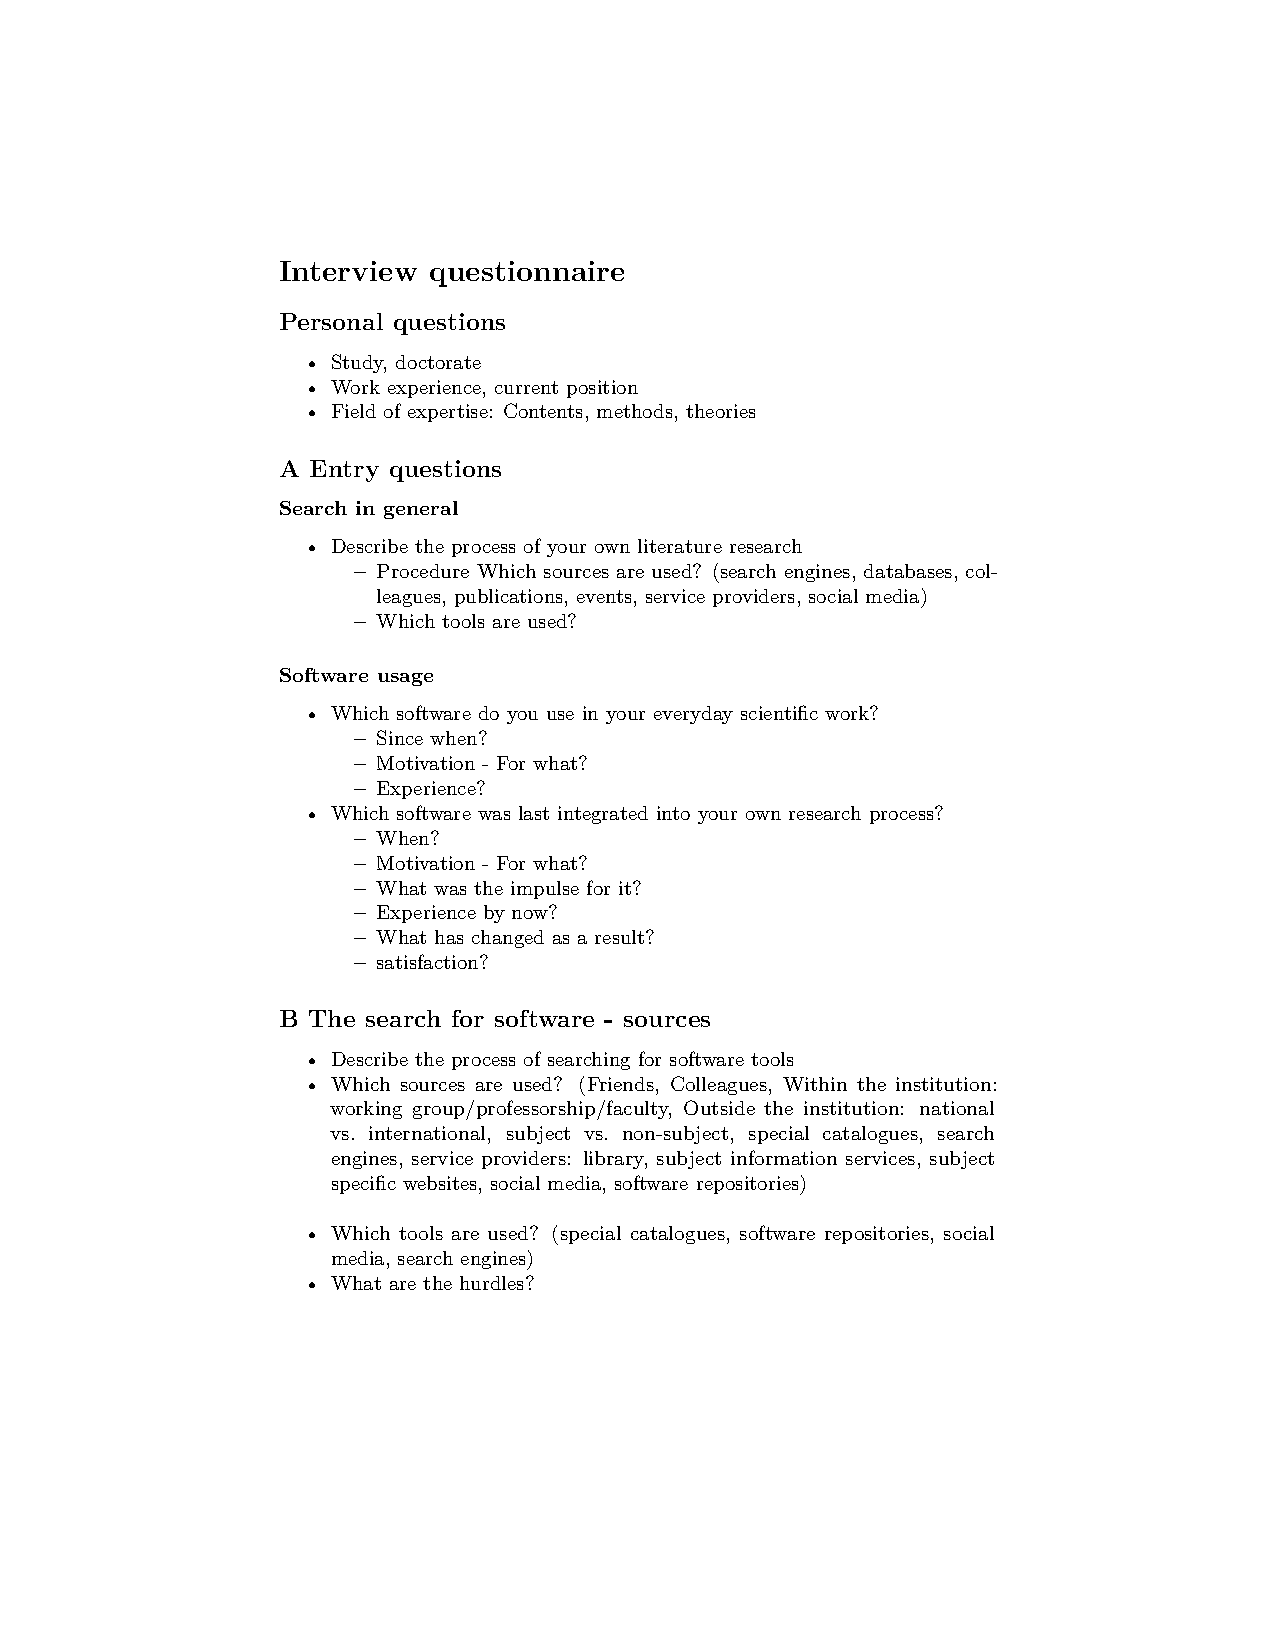
\includepdf[pages=-,pagecommand={\thispagestyle{empty}}]{_methods/Interview_guidelines_en.pdf}
\cleardoublepage

\chapter{Category System}
\label{sec:Category_system}
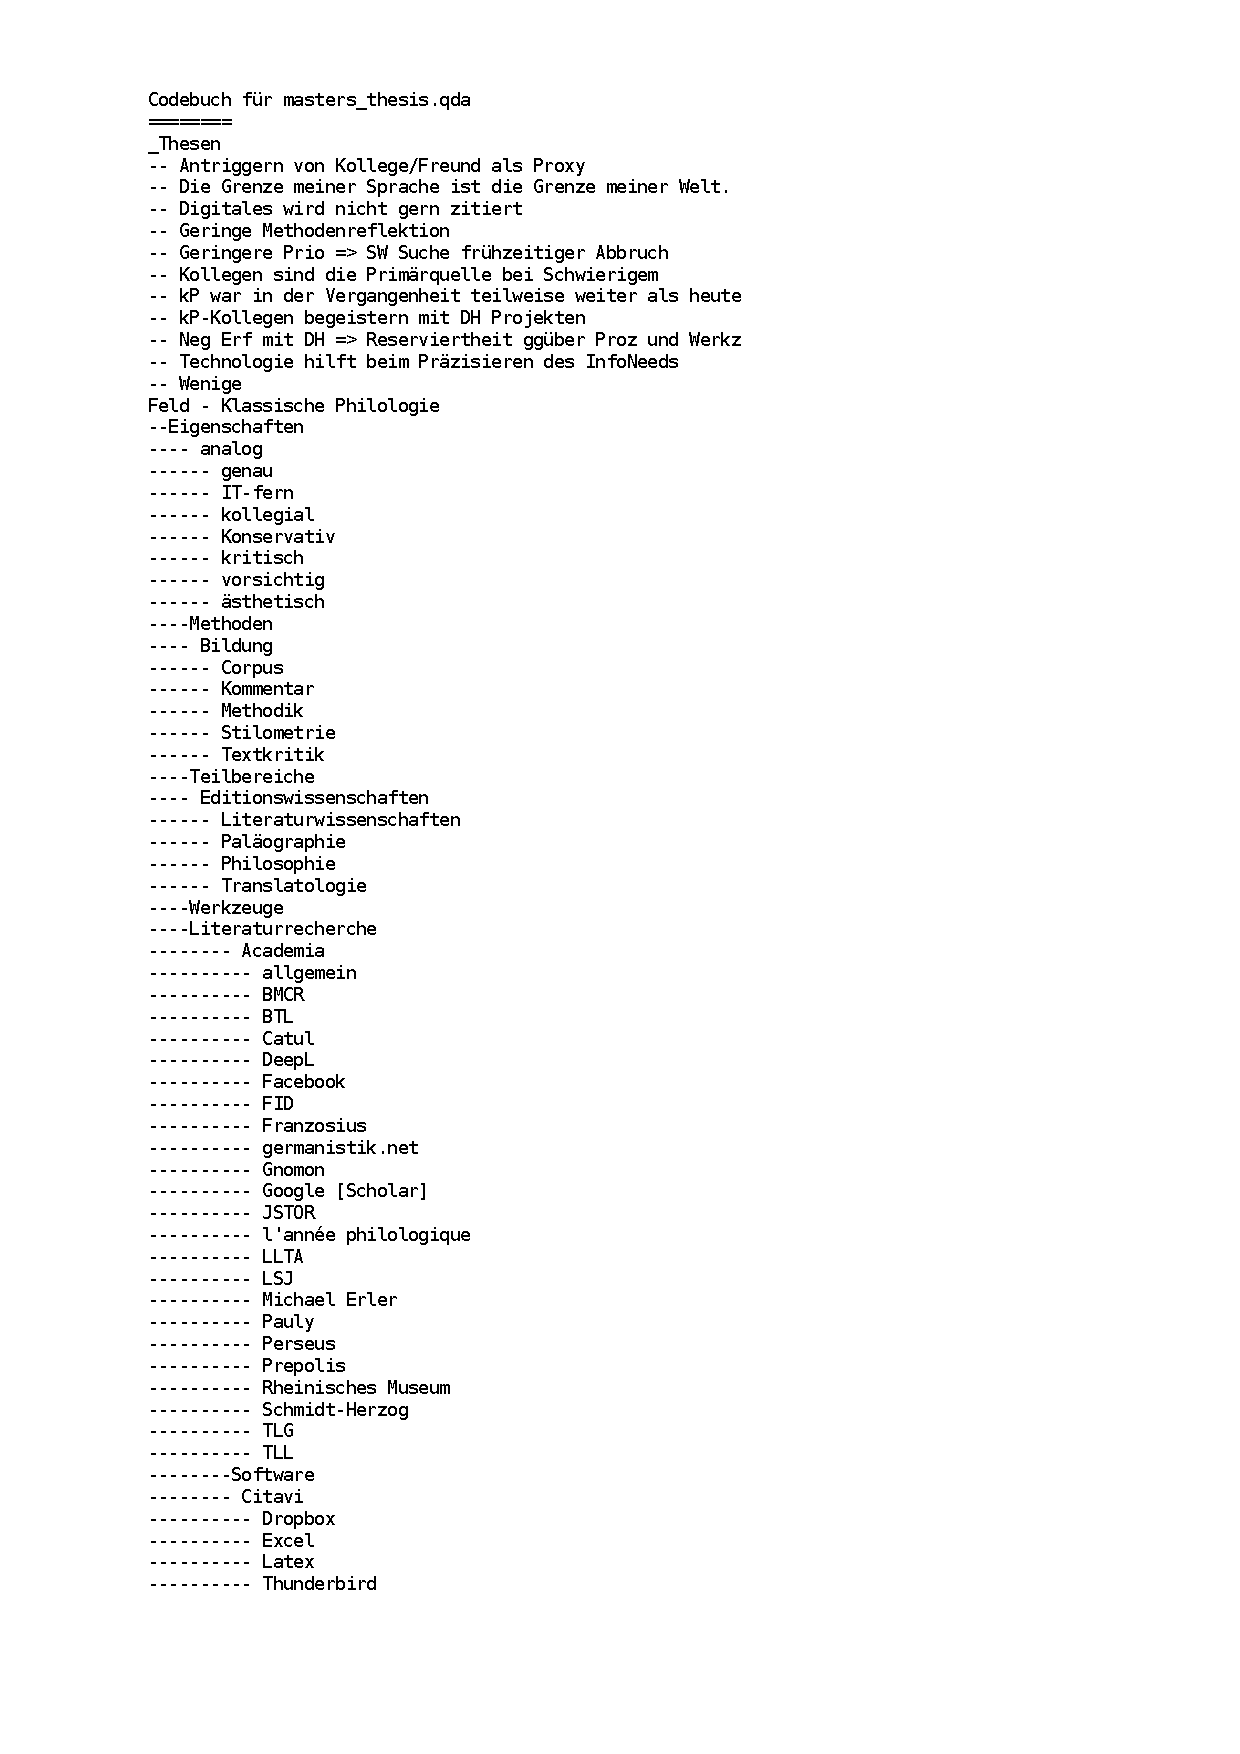
\includepdf[pages=-,pagecommand={\thispagestyle{empty}}]{_analysis/codebook.txt.pdf}
\cleardoublepage

\chapter{Consent Form}
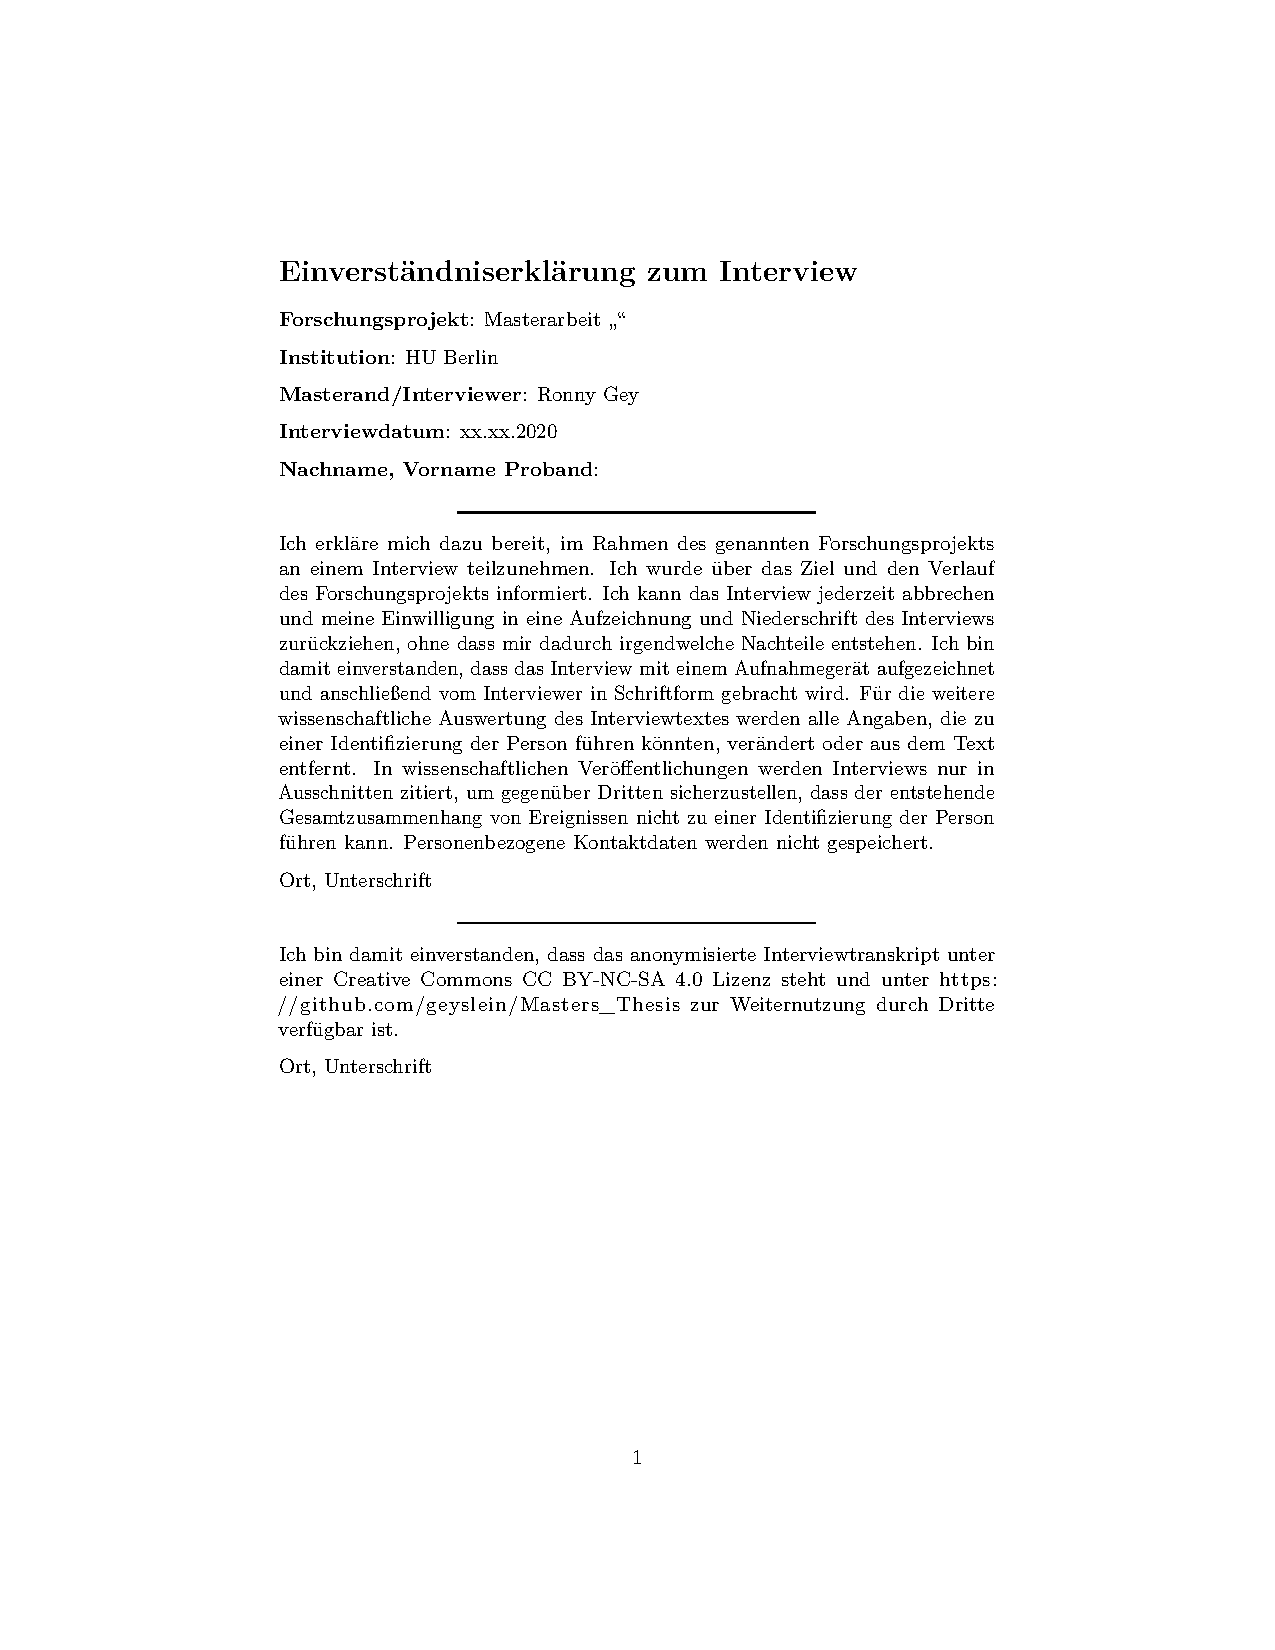
\includepdf[pages=-,pagecommand={\thispagestyle{empty}}]{_data/collection/consent form interview (German).pdf}

\end{appendices}
%======================================================================
%	Selbstständikeitserklärung
%======================================================================
\includepdf[pages=-,pagecommand={\thispagestyle{empty}}]{_admin/Selbststaendigkeitserklaerung_ohneU}
\cleardoublepage

\end{document}